\documentclass[12pt]{article}

\usepackage{amssymb}
\usepackage{physics}
\usepackage{hyperref} % for hyperlinks in references
\usepackage[notref,notcite,color]{showkeyskay}\definecolor{labelkey}{rgb}{1,0,0.5}

\usepackage{graphicx}
\usepackage{caption} % for \caption*
\usepackage{mdframed} % for framed text and formulas
\usepackage[dvipsnames]{xcolor}

\numberwithin{equation}{section}

\newcommand{\be}{\begin{equation}}
\newcommand{\ee}{\end{equation}}
\newcommand{\e}{\mbox{e}}
\newcommand {\mm}[1]{\quad\mbox{#1}\quad}
\newcommand {\MM}[1]{\qquad\mbox{#1}\qquad}

\textwidth 180mm
\textheight 230mm
\voffset = -20mm
\hoffset = -10mm

\title{Overview: a cell fluid model with Curie-Weiss interaction}

\author{R.V.~Romanik
	\\ \small Institute for Condensed Matter Physics, NAS of Ukraine
	\\ \small 1~Svientsitskii Street, 79011, Lviv, Ukraine
	\\ \small romanik@icmp.lviv.ua}
%\author{R.V.~Romanik \\ Institute for Condensed Matter Physics, NAS of Ukraine}

\begin{document}
	
	\maketitle
	
	%\begin{multicols}{2}
	
	\abstract{Review of the cell fluid model with Curie-Weiss interaction.
		\\	
		\textbf{Keywords:} Cell fluid model, Curie-Weiss interaction.
	}
	
	\tableofcontents
	
	\section{Introduction}
	The cell model was introduced and described in~\cite{KKD18,KKD20}. This model possesses an exact solution in the case of Curie-Weiss interaction. The exact asymptotic expression for the grand partition function was obtained in~\cite{KKD20}.
	The goal of this manuscript is to summarize the notation, properly account for quantity dimensions corresponding to physical problems.
	
	\section{\label{sec:model} Model}
	Let us briefly introduce the model, the notation, and then summarize the known results for the model.
	
	The main results are obtained within the formalism of the grand canonical ensemble. An open system of point particles is considered in volume $V$. The total volume $V$ is divided into $N_v$ congruent cubic cells $\Delta_l$ of volume $v=c^3$ each, such that the volume $V$ is the union of all $\Delta_l$
	\begin{equation*}
		V = \bigcup_{l=1}^{N_v}\Delta_l,
	\end{equation*}
	and for each pair of $\Delta_l$ and $\Delta_m$
	\begin{equation*}
		\Delta_l \cap \Delta_m = \emptyset, \text{ if } l \neq m.
	\end{equation*}
	
	\textbf{Interaction.} The interaction energy between particles in configuration $\gamma = \{x_1, ..., x_N\}$, where $x_i$ is the space coordinate of the $i$-th particle and $N$ is the number of points (particles) in the configuration $\gamma$, is defined as follows
	\begin{equation*}
		W_{N_v}(\gamma) = \frac{1}{2} \sum_{x,y \in \gamma} \Phi_{N_v} (x,y)
	\end{equation*}
	where $\Phi_{N_v}$ is given by the Curie-Weiss interaction
	\begin{equation}
		\label{def:curie-weiss-pot}
		\Phi_{N_v}(x, y) = -\frac{J_1}{N_v} + J_2\sum_{l=1}^{N_v} I_{\Delta_l}(x) I_{\Delta_l}(y),
	\end{equation}
	and $I_{\Delta_l}(x)$ is the indicator of $\Delta_l$
	\begin{equation}
		\label{def:I}
		I_{\Delta_l} (x) = \left\{
		\begin{array}{ll}
			1, \quad x \in \Delta_l,
			\\
			0, \quad x \notin \Delta_l.
		\end{array}
		\right.
	\end{equation}
	The first term in $\Phi_{N_v}$ describes the pairwise attraction between all particles and is characterized by $J_1 > 0$. The second term in $\Phi_{N_v}$ describes the repulsion between two particles contained within the same cell $\Delta_l$ and is characterized by $J_2 > 0.$ For convenience, in $W_{N_v}$ above the self-interaction term $\Phi_{N_v}(x,x)$ is included, which does not affect the physics of the model. Two cases are possible, either two particles belong to the same cell or to different ones. Explicitly, one has
	\begin{equation}
		\Phi_{N_v}(x, y) = \left\{
		\begin{array}{ll}
			-\frac{J_1}{N_v} + J_2, & \text{when particles are in the same cell,}
			\\
			-\frac{J_1}{N_v}, & \text{otherwise.}
		\end{array}
		\right.
	\end{equation}
	In~\cite{KKD20}, the notation $\abs{\gamma}$ was used to denote the number of points (particles) in configuration $\gamma$, thus $\abs{\gamma} \equiv N$.
	
	\begin{mdframed}[linecolor=black,linewidth=1pt,leftline=true]
	If the notation from~\cite{HansenMcDonald13} is followed, the previous formulas can be rewritten as follows. The space coordinate of the $i$-th particle is denoted by $\vb{r}_i$, and thus the configuration of $N$ particles is defined by $\gamma = \{\vb{r}^N\}$, where $\vb{r}^N \equiv \vb{r}_1, ..., \vb{r}_N$. The interaction energy is expressed as (cf.~\cite[eq.~(2.5.16)]{HansenMcDonald13})
	\begin{eqnarray*}
		W_{N_v}(\vb{r}^N) & = & \frac{1}{2} \sum_{\vb{r}_i,\vb{r}_j \in \gamma} \Phi_{N_v} (\vb{r}_i,\vb{r}_j).
		\\
		& = & \frac12 {\sum_{i=1}^N \sum_{j=1}^N} \Phi_{N_v} (\vb{r}_i,\vb{r}_j),
	\end{eqnarray*}
	with
	\begin{equation*}
		\Phi_{N_v}(\vb{r}_i, \vb{r}_j) = -\frac{J_1}{N_v} + J_2\sum_{l=1}^{N_v} I_{\Delta_l}(\vb{r}_i) I_{\Delta_l}(\vb{r}_j),
	\end{equation*}
	and
	\begin{equation*}
		I_{\Delta_l} (\vb{r}) = \left\{
		\begin{array}{ll}
			1, \quad \vb{r} \in \Delta_l,
			\\
			0, \quad \vb{r} \notin \Delta_l.
		\end{array}
		\right.
	\end{equation*}
	Unlike~\cite[eq.~(2.5.16)]{HansenMcDonald13}, we do not exclude term with $i = j$ in the expression for $W_{N_v}$ due to the self-interaction.
	\end{mdframed}
	
	\textbf{Stability.} For stability of interaction the following condition must hold
	\begin{equation*}
		J_2 > J_1
	\end{equation*}
	to satisfy the following inequality~\cite{KKD20,Ruelle70}
	\begin{equation}
		\int_{V} \Phi_{N_v}(x,y) {\rm d}y > 0, \quad \text{for all } x \in V.
	\end{equation}
	Note that there is one contribution to this integral from a cell containing the coordinate $x$, and $(N_v - 1)$ contributions from the other cells:
	\begin{eqnarray*}
		\int_{V} \Phi_{N_v}(x,y) {\rm d}y & = & \left(-\frac{J_1}{N_v} + J_2\right)v - (N_v - 1) \frac{J_1}{N_v}v
		\\
		& = & (J_2 - J_1)v > 0.
	\end{eqnarray*}
	The ratio of the two energy constants is denoted by
	$$a = J_2/J_1,$$
	and thus $a > 1.$
	
	\textbf{The grand partition function} (GPF) is expressed as follows~\cite[eqs.~(2.4.6) and~(2.3.13)]{HansenMcDonald13}
	\begin{equation*}
		\Xi = \sum_{N=0}^{\infty}\frac{z^N}{N!} \int_{V} \dotsc \int_{V} \exp(-\beta W_{N_v}(\gamma)) {\rm d} x_1 \dotsc {\rm d} x_N
	\end{equation*}
	where $z$ is the activity
	\begin{equation*}
		z = \frac{\exp(\beta \mu)}{\Lambda^3},
	\end{equation*}
	$\beta = 1/(k_{\rm B} T)$ the inverse temperature, $k_{\rm B}$ the Boltzmann constant, $T$ the temperature, $\mu$ the chemical potential, $\Lambda = (2\pi\beta\hbar^2/m)^{1/2}$ the de Broglie thermal wavelength, $\hbar$ the Planck constant, $m$ the mass of a particle. In GPF the integration goes over all configurations with $N$ particles and then the summation goes over all positive integer values of $N$.
	
	\begin{mdframed}[linecolor=black,linewidth=1pt,leftline=true]
		Alternatively, in notation from~\cite{HansenMcDonald13}, the GPF is expressed as [cf. eqs.~(2.4.6) and~(2.3.13)]
		\begin{equation}\label{ZGR}
			\Xi=\sum_{N=0}^{\infty}\frac{z^N}{N!}Z_N,
		\end{equation}
		where $Z_N$ is the configuration integral:
		\begin{equation}
			Z_N = \int\exp(-\beta W_{N_v}(\vb{r}^N)){\rm d}\vb{r}^N
		\end{equation}
		with ${\rm d} \vb{r}^N \equiv {\rm d}{\vb r_1} \dotsc {\rm d}{\vb r_N}$.
	\end{mdframed}
	
	\textbf{Reduced quantities.} Natural units for energy and length in the model are $J_1$ and $c$, respectively. It is standard practice to express thermodynamic results in terms of dimensionless quantities normalized by these natural units. The advantage of using such quantities is that their numerical values are typically of the order of unity, which simplifies analysis. Thus, we introduce the following reduced quantities:
	%the reduced temperature $T^* = k_{\rm B} T / J_1$, the reduced inverse temperature $p = \beta J_1$, reduced chemical potential $\mu^* = \mu / J_1$, and the reduced pressure $P^* = Pv/J_1$.
	\begin{eqnarray}
		\label{def:reduced}
		T^* := \frac{k_{\rm B} T}{J_1} & \quad & \text{ -- the reduced temperature;} 
		\nonumber\\
		p := \beta J_1 = \frac{1}{T^*} & \quad & \text{ -- the reduced inverse temperature;}
		\nonumber\\
		\mu^* := \frac{\mu}{J_1} & \quad & \text{ -- the reduced chemical potential;}
		\nonumber\\ 
		P^* := \frac{Pv}{J_1} & & \text{ -- the reduced pressure;}
		\nonumber\\
		S^* := \frac{S}{k_{\rm B} \langle N \rangle} & & \text{ -- the reduced entropy;}
		\nonumber\\
		\rho^* := \frac{\langle N \rangle}{V} v && \text{ -- the reduced (particle number) density.}
	\end{eqnarray}
	For any dimensional quantity $Q$, it is convenient to denote its reduced counterpart by $Q^*$. To maintain consistency with other thermodynamic quantities, it may be beneficial to use $\beta^*$ instead of $p$ for the reduced inverse temperature (cf.~\cite{RDGMR13}).
	
	\subsection{Partition function transformation}
	Note the following summation:
	\begin{equation}
		\sum_{x,y \in \gamma} 1 = N^2 = \abs{\gamma}^2.
	\end{equation}
	The GPF is then explicitly written as
	\begin{equation}
		\label{eq:gpf1}
		\Xi = \sum_{N=0}^{\infty} \frac{\Lambda^{-3N}}{N!}\int \exp[\beta\mu N + \frac{p}{2N_{v}} N^2 - \frac{ap}{2} \sum_{x,y \in \gamma} \sum_{l=1}^{N_v} \mathbb{I}_{\Delta_l}(x)\mathbb{I}_{\Delta_l}(y)] {\rm d} x_1 \dotsc {\rm d} x_N.
	\end{equation}
	
	\begin{mdframed}[linecolor=black,linewidth=1pt,leftline=true]
	Alternatively
		\begin{equation}
			\label{eq:gpf1_alt}
			\Xi = \sum_{N=0}^{\infty} \frac{\Lambda^{-3N}}{N!}
			\int
			\exp[\beta\mu N + \frac{\beta^*}{2N_{v}} N^2 - \frac{a\beta^*}{2} \sum_{\vb{r}_i,\vb{r}_j \in \gamma} \sum_{l=1}^{N_v} \mathbb{I}_{\Delta_l}(\vb{r}_i)\mathbb{I}_{\Delta_l}(\vb{r}_j)] {\rm d} \vb{r}^N.
		\end{equation}
	\end{mdframed}
	Equations~\eqref{eq:gpf1} and~\eqref{eq:gpf1_alt} can be compared with~\cite[(2.5)]{KKD20}.
	
	For a given $l = 1, \cdots , N_v$ and a configuration $\gamma$, we set $\gamma_l = \gamma \cap \Delta_l,$ that is, $\gamma_l$ is the part of the configuration contained in $\Delta_l$. Then, $N_l$ or $\abs{\gamma_l}$ stands for the number of points (particles) of $\gamma$ contained in $\Delta_l$.
	
	\textbf{Some useful formulas}. Note the following summation results:
	\begin{equation}
		\label{eq:1}
		N_l \equiv \abs{\gamma_l} = \sum_{x \in \gamma_l} 1 = \sum_{x \in \gamma} \mathbb{I}_{\Delta_l}(x) = \sum_{j=1}^{N} \mathbb{I}_{\Delta_{l}}(x_j),
	\end{equation}
	\textbf{\textcolor{Red}{Question:}} Can $x \in \gamma_l$ and $x \in \Delta_l$ be used interchangeably?
	\begin{equation}
		\label{eq:2}
		\sum_{l=1}^{N_v} N_l = N, \quad \sum_{l=1}^{N_v} \abs{\gamma_l} = \abs{\gamma},
	\end{equation}
	\begin{equation}
		\label{eq:3}
		\left(\sum_{l=1}^{N_v} N_l \right)^2 = N^2, \quad \left(\sum_{l=1}^{N_v} \abs{\gamma_l} \right)^2 = \abs{\gamma}^2.
	\end{equation}
	\begin{equation}
		\label{eq:4}
		\sum_{x \in \gamma} \rightarrow \sum_{l=1}^{N_v} \sum_{x \in \Delta_l};
	\end{equation}
	\begin{equation}
		\label{eq:5}
		\sum_{x,y \in \gamma} \rightarrow \sum_{l,l'=1}^{N_v} \sum_{x \in \Delta_l} \sum_{y \in \Delta_{l'}}.
	\end{equation}
	\begin{equation}
		\label{eq:6}
		\sum_{x \in \Delta_l}\sum_{y \in \Delta_l'} 1 = N_l N_{l'} = \abs{\gamma_l} \abs{\gamma_{l'}}.
	\end{equation}
	\begin{equation}
		\label{eq:sumII}
		\sum_{x,y \in \gamma}\sum_{l=1}^{N_v} \mathbb{I}_{\Delta_l}(x) \mathbb{I}_{\Delta_{l}}(y) = \sum_{l=1}^{N_v} N_l^2 \equiv \sum_{l=1}^{N_v} \abs{\gamma_l}^2.
	\end{equation}
	Combining these formulas, we get
	\begin{eqnarray}
		\sum_{x,y \in \gamma} \Phi_{N_v}(x,y) & = & \sum_{l,l'=1}^{N_v} \sum_{x \in \Delta_l} \sum_{y \in \Delta_{l'}} \Phi_{N_v}(x,y)
		\nonumber\\
		& = & - \frac{J_1}{N_v} \left(\sum_{l=1}^{N_v} N_l\right)^2 + J_2\sum_{l=1}^{N_v}N_l^2
		\\
		& = & - \frac{J_1}{N_v} \left(\sum_{l=1}^{N_v} \abs{\gamma_l}\right)^2 + J_2\sum_{l=1}^{N_v}\abs{\gamma_l}^2
	\end{eqnarray}
	
	\textbf{GPF transformation}. To rewrite the integrand in~\eqref{eq:gpf1} in a more convenient form we set (cf.~\cite[eq.~(2.7)]{KKD20})
	\begin{equation}
		F_{N_v}(\varrho, p, \mu) = \exp[\frac{p}{2N_v}\left(\sum_{l=1}^{N_v} \varrho_l\right)^2 + \beta\mu\sum_{l=1}^{N_v} \varrho_l - \frac{a p}{2} \sum_{l=1}^{N_v} \varrho_l^2],
	\end{equation}
	where $\varrho \in \mathbb{N}_0^N$ is a vector with nonnegative integer components $\varrho_l$, $l=1, 2, \ldots , N_v$, i.e. $\varrho = (\varrho_1, \varrho_2, \ldots, \varrho_{N_{v}})$.
	
	For $\varrho$, we substitute the vector $\nu(\gamma) \in \mathbb{N}_0^N$ with components $N_l$ (or $\abs{\gamma_l}$), which have the meaning of the number of points in a cell $\Delta_{l}$ in cofiguration $\gamma$, i.e. $\nu(\gamma)=(N_1, N_2, \ldots, N_{N_v})$ or $\nu(\gamma) = (\abs{\gamma_1}, \abs{\gamma_2}, \ldots, \abs{\gamma_{N_v}})$, and obtain the following expression for the GPF in~\eqref{eq:gpf1}:
	\begin{equation}
		\Xi = \sum_{N=0}^{\infty} \frac{\Lambda^{-3N}}{N!}\int_{V^N} F_{N_v}(\nu(\gamma),p,\mu) {\rm d} x_1 \dotsc {\rm d} x_N,
	\end{equation}
	which can be compared with~\cite[eq.~(2.8)]{KKD20}.
	
	The next step is to intorduce the Kronecker $\delta$-symbol for $n, m \in \mathbb{N}_0$ as
	\begin{equation}
		\delta_{nm} = \int_0^1 \exp[2\pi {\rm i} t (n-m)] {\rm d}t
	\end{equation}
	and rewrite $F_{N_v}$ as
	\begin{equation}
		F_{N_v}(\nu(\gamma),p,\mu) = \sum_{\varrho \in \mathbb{N}_0^{N_v}} F_{N_v}(\varrho, p, \mu) 
		\int\limits_{[0,1]^{N_v}} \exp[2\pi{\rm i} \sum_{l=1}^{N_v} (\varrho_l - N_l)t_l ] {\rm d} t_1 \ldots {\rm d} t_{N_v},
	\end{equation}
	to arrive at (cf.~\cite[(2.9)]{KKD20})
	\begin{eqnarray}
		\label{eq:XiR}
		\Xi & = &  \sum_{\varrho \in \mathbb{N}_0^{N_v}} F_{N_v}(\varrho, p, \mu) 
		\sum_{N=0}^{\infty} \frac{\Lambda^{-3N}}{N!} 
		\nonumber\\
		&& \times \int\limits_{V^N} \int\limits_{[0,1]^{N_v}} 
		\exp[2\pi{\rm i} \sum_{l=1}^{N_v} (\varrho_l - N_l)t_l ] {\rm d} t_1 \ldots {\rm d} t_{N_v} {\rm d}x_1 \ldots {\rm d}x_N 
		\nonumber\\
		& = & \sum_{\varrho \in \mathbb{N}_0^{N_v}} F_{N_v}(\varrho, p, \mu)
		\int\limits_{[0,1]^{N_v}} \exp(2\pi{\rm i} \sum_{l=1}^{N_v} \varrho_l t_l) R_{N_v}(t_1, \ldots, t_{N_v}) {\rm d} t_1 \ldots {\rm d} t_{N_v}.
	\end{eqnarray}
	The summation over $\varrho$ is understood as
	\begin{equation}
		\sum_{\varrho \in \mathbb{N}_0^{N_v}} = \sum_{\varrho_1=0}^{\infty} \ldots \sum_{\varrho_{N_v}=0}^{\infty}.
	\end{equation}
	The quantity $R_N$ is expressed as follows (cf.~\cite[(2.10)]{KKD20})
	\begin{eqnarray}
		\label{def:RN}
		R_{N_v}(t_1, \ldots, t_{N_v}) & = & \sum_{N=0}^{\infty} \frac{\Lambda^{-3N}}{N!} \int\limits_{V^N} \exp(-2\pi{\rm i} \sum_{l=1}^{N_v} N_l t_l) {\rm d}x_1 \ldots {\rm d}x_N
		\nonumber\\
		&=& \sum_{N=0}^{\infty} \frac{\Lambda^{-3N}}{N!} \int\limits_{V^N} \exp(-2\pi{\rm i} \sum_{l=1}^{N_v} \sum_{j=1}^{N} \mathbb{I}_{\Delta_{l}}(x_j) t_l) {\rm d}x_1 \ldots {\rm d}x_N,
	\end{eqnarray}
	We used~\eqref{eq:1} to get the last line in the above equation.
	
	Note that the expression under the integral in the last line of~\eqref{def:RN} is factorized in $j$:
	\begin{eqnarray}
		R_{N_v}(t_1, \ldots, t_{N_v}) & = & \sum_{N=0}^{\infty}\frac{1}{N!} 
		\left\{\frac{1}{\Lambda^{3}} \int\limits_V \exp[-2\pi{\rm i}\sum_{l=1}^{N_v} \mathbb{I}_{\Delta_{l}}(x) t_l] {\rm d}x \right\}^N.
	\end{eqnarray}
	Applying the following transformation for the integral over $V$
	\begin{equation}
		\int\limits_V \ldots {\rm d}x = \sum_{l=1}^{N_v}\int\limits_{\Delta_l} \ldots {\rm d}x,
	\end{equation}
	and taking into account the definition of $\mathbb{I}_{\Delta_l}$~\eqref{def:I}, one gets for $R_{N_v}$
	\begin{eqnarray}
		\label{eq:RNL}
		R_{N_v}(t_1, \ldots, t_{N_v}) & = & \sum_{N=0}^{\infty}\frac{1}{N!} \left[ \frac{1}{\Lambda^3} \sum_{l=1}^{N_v} \int\limits_{\Delta_l} \exp(-2\pi{\rm i}t_l) {\rm d}x \right]^N
		\nonumber\\
		&=& \exp[\frac{v}{\Lambda^3} \sum_{l=1}^{N_v} \exp(-2\pi{\rm i} t_l)].
	\end{eqnarray}
	Here we used an obvious result $\int_{\Delta_l} {\rm d}x = v$. It is natural to introduce
	\begin{equation}
		v^* = \frac{v}{\Lambda^3},
	\end{equation}
	and write down the final expression for $R_{N_v}$
	\begin{equation}
		\label{eq:RNv}
		R_{N_v}(t_1, \ldots, t_{N_v}) = \exp[v^* \sum_{l=1}^{N_v} \exp(-2\pi{\rm i} t_l)].
	\end{equation}
	Compare this expression with the corresponding one in~\cite[p.~4]{KKD20} 
	
	Let us substitute~\eqref{eq:RNv} into~\eqref{eq:XiR}
	\begin{equation}
		\label{eq:XiIntt}
		\Xi(p,\mu) = \sum_{\varrho \in \mathbb{N}_0^{N_v}} F_{N_v}(\varrho, p, \mu) \prod\limits_{l=1}^{N_v} \int\limits_{0}^{1} \exp[2\pi{\rm i}\varrho_l t_l + v^* \exp(-2\pi{\rm i} t_l)] {\rm d} t_l.
	\end{equation}
	Here, the integral gives the following result:
	\begin{equation}
		\label{integral1}
		\int\limits_{0}^{1} \exp[2\pi{\rm i}\varrho_l t_l + v^* \exp(-2\pi{\rm i} t_l)] {\rm d} t_l = \frac{{(v^*)}^{\varrho_l}}{\varrho_l !}.
	\end{equation}
	\textbf{\textcolor{Red}{NOTE:}} This integral has not been explicitly written down in any of the papers~\cite{KKD18, KKD20, KD22}, and I do not know how it is calculated. However, I have determined that this result was implicitly substituted into~\cite[(2.11)]{KKD20}. I have verified this using Maple, and it yields the result given in~\eqref{integral1}.
	
	The GPF takes on the form (cf.~\cite[2.11]{KKD20}):
	\begin{eqnarray}
		\label{eq:XiPi}
		\Xi(p,\mu) & = & \sum_{\varrho \in \mathbb{N}_0^{N_v}} F_{N_v}(\varrho, p, \mu) \prod\limits_{l=1}^{N_v} \frac{(v^*)^{\varrho_l}}{\varrho_l !}
		\nonumber\\
		& = & \sum_{\varrho \in \mathbb{N}_0^{N_v}} \exp[\frac{p}{2 N_v} \left(\sum_{l=1}^{N_v} \varrho_l\right)^2] \prod\limits_{l=1}^{N_v} \pi(\varrho_l, \mu),
	\end{eqnarray}
	where
	\begin{equation}
		\label{def:pirho}
		\pi(\varrho_l, \mu) = \frac{(v^*)^{\varrho_l}}{\varrho_l !} \exp(\beta\mu\varrho_l - \frac{ap}{2}\varrho_l^2), \quad \varrho_l \in \mathbb{N}_0.
	\end{equation}
	\begin{mdframed}[linecolor=black,linewidth=1pt,leftline=true]
		In a generic form
		\begin{equation}
			\label{def:pin}
			\pi(n, \mu) = \frac{(v^*)^n}{n!} \exp(\beta\mu n - \frac{ap}{2}n^2), \quad n \in \mathbb{N}_0.
		\end{equation}
	\end{mdframed}
	
	\textbf{The Poisson distribution} results from~\eqref{def:pin} at $p=0$, i.e. in the high-temperature limit. To see this, rewrite expression for $\pi(n,\mu)|_{p=0}$ as
	\begin{equation}
		\pi(n,\mu)|_{p=0} = {\rm e}^{v^* {\rm e}^{\beta\mu}} 
		\frac{\left(v^* {\rm e}^{\beta\mu}\right)^n}{n!} {\rm e}^{-v^* {\rm e}^{\beta\mu}} 
		= {\rm e}^{v^* {\rm e}^{\beta\mu}} f(n; \lambda)
	\end{equation}
	where the (non-normalized) Poisson distribution $f(n; \lambda)$ is given by
	\begin{equation}
		f(n; \lambda) = \frac{\lambda^n {\rm e}^{-\lambda}}{n!}, \quad \lambda = v^* {\rm e}^{\beta\mu}.
	\end{equation}
	
	\textbf{Further transformation}. Applying the Gaussian integral
	\begin{equation}
		\int\limits_{-\infty}^{\infty} {\rm e}^{-\alpha y^2 + \beta y} {\rm d}y = \sqrt{\frac{\pi}{\alpha}} {\rm e}^{\frac{\beta^2}{4\alpha}},
	\end{equation}
	explicitly to Eq.~\eqref{eq:XiPi}
	\begin{equation}
		\label{eq:gaussInt}
		\exp[\frac{p}{2N_v}\left(\sum_{l=1}^{N_v} \varrho_l\right)^2] = \sqrt{\frac{N_v}{2\pi p}}
		\int\limits_{-\infty}^{\infty} \exp(-N_v \frac{y^2}{2p} + y\sum_{l=1}^{N_v} \varrho_l) {\rm d}y
	\end{equation}
	we transform~\eqref{eq:XiPi} into the following expression
	\begin{equation}
		\label{eq:XiInty}
		\Xi (p, \mu) = \sqrt{\frac{N_v}{2\pi p}} \int\limits_{-\infty}^{\infty} \exp[N_v E(y, p, \mu)] {\rm d} y,
	\end{equation}
	where 
	\begin{equation}
		\label{def:E}
		E(y,p,\mu) = -\frac{y^2}{2p} + \ln K_0(y,p,\mu),
	\end{equation}
	with
	\begin{equation}
		\label{def:K}
		K_0(y,p,\mu) = \sum_{n=0}^{\infty} \frac{(v^*)^n}{n!} \exp[(y+\beta\mu)n - \frac{ap}{2}n^2].
	\end{equation}
	Explicit derivation of expressions for $E(y,p,\mu)$ and $K_0(y,p,\mu)$ is given in Appendix~\ref{sec:app1}.
	
	\begin{mdframed}[linecolor=black,linewidth=1pt,leftline=true]
	Often, it is convenient to express all the expressions in reduced quantities from~\eqref{def:reduced}, thus we will write the version for important quantities in reduced units as well:
	\begin{equation}
		\label{def:reducedE}
		E(y,T^*,\mu^*) = -\frac{1}{2}T^* y^2 + \ln K_0(y, T^*, \mu^*),
	\end{equation}
	\begin{equation}
		K_0(y,T^*,\mu^*) = \sum_{n=0}^{\infty} \frac{(v^*)^n}{n!} \exp[\left(y+\frac{\mu^*}{T^*}\right)n - \frac{a}{2T^*}n^2].
	\end{equation}
	\end{mdframed}
	
	\textbf{Some reasoning on numerical value of $v^*$.} During particular calculations, a numerical value for $v^*$ must be chosen. Which value to select may depend on physical reasoning. The dependence of results on $v^*$ may also be investigated.
	
	Since $v^* = c^3/\Lambda^3$, we may focus on a choice for $c$. One approach to choosing $c$ is in such a way that a classical consideration is justified. For example, it can be taken as the mean nearest-neighbour separation, see~\cite[Sec.~1.1]{HansenMcDonald13}. From the data given in~\cite[Table~1.1]{HansenMcDonald13}, the ratio $c/\Lambda$ may vary between $3.8$ and $59$ (we ignored data for $H_2$, as quantum effects are important for this substance). This defines possible values for $v^*$ as ranging between $57$ and $2 \cdot 10^5$.
	
	\textbf{Constraint on $E(y,p,\mu)$}. From inequality
	\begin{equation}
		\left(\frac{y+\beta\mu}{ap} - n\right)^2 \geq 0
	\end{equation}
	it follows
	\begin{equation}
		(y+\beta\mu)n - \frac{ap}{2}n^2 \leq \frac{(y+\beta\mu)^2}{2ap}.
	\end{equation}
	The last inequality, in turn, leads to corresponding inequalities for $K(y,p,\mu)$
	\begin{eqnarray}
		K_0(y,p,\mu) & \leq & \sum_{n=0}^{\infty}\frac{(v^*)^n}{n!} \exp[\frac{(y+\beta\mu)^2}{2ap}]
	\end{eqnarray}
	or
	\begin{equation}
		K_0(y,p,\mu) \leq \exp[\frac{(y+\beta\mu)^2}{2ap}] \exp(v^*),
	\end{equation}
	and for $E(y,p,\mu)$
	\begin{equation}
		\label{ineq:E0}
		E(y,p,\mu) \leq -\frac{a-1}{2ap}y^2 + \frac{\beta\mu}{2ap}(2y+\beta\mu) + v^*.
	\end{equation}
	Since $a>1$, \eqref{ineq:E0} implies the following limits for fixed $p$ and $\mu$
	\begin{equation}
		\lim_{y \to -\infty} E(y,p,\mu) = -\infty, \quad \lim\limits_{y \to +\infty} E(y,p,\mu) = -\infty.
	\end{equation}
	Typical behavior of $E(y,p,\mu)$ as a function of $y$ in the single-phase domain is illustrated in Fig.~\ref{fig:E0_vs_y}
	\begin{figure}[htbp]
		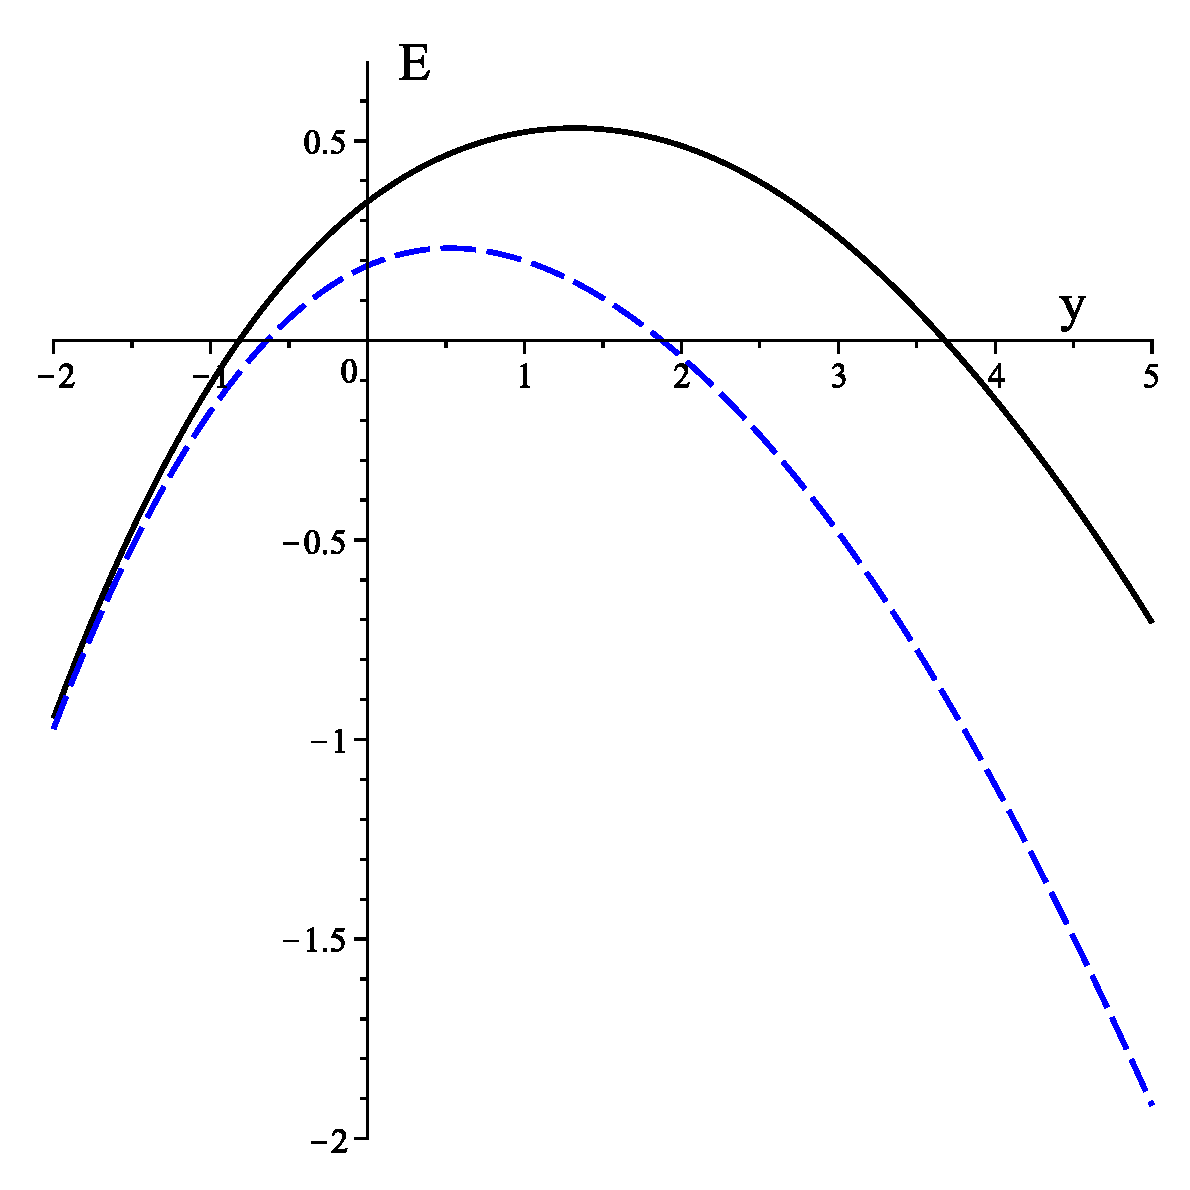
\includegraphics[width=0.5\textwidth,angle=0]{E0_vs_y2}
		\centering
		\captionsetup{width=0.6\textwidth}
		\caption{Quantity $E(y,p,\mu)$ as a function of $y$ at $p=2.0$ ($T^*=0.5$) and $\beta\mu=-2.0$ ($\mu^*=-1.0$) for two different values of $v^*$: Solid line (black): $v^* = 10$, Dash line (blue): $v^* = 5$.}
		\label{fig:E0_vs_y}
	\end{figure}
	
	\textit{Remark}. The estimate in~\eqref{ineq:E0} implies the following: (a) the integral in~\eqref{eq:XiInty} converges for all $p>0$ and $\mu \in \mathbb{R}$, as $a>1$; (b) for fixed $p$ and $\mu$, since $E(y,p,\mu)$ is bounded above, it has global maxima, each of which is also a local maximum.
	
	\textbf{Note on numerical values for parameters.} If not specified otherwise, the following numerical values for parameters of the model are used for calculations and graphical representation of results:
	\begin{equation}
		v^* = 5.0; \quad a = 1.2.
	\end{equation}
	
	
	\section{Pressure}
	By the known thermodynamic formula (cf.~\cite[(2.16)]{KKD20})
	\begin{equation}
		\label{def:eos}
		%P V = k_{\rm B} T \ln \Xi(\beta, \mu)
		P V = \beta^{-1} \ln \Xi(\beta, \mu)
	\end{equation}
	where $P$ is the pressure. To calculate the large $N_v$ limit in~\eqref{eq:XiInty} we first determine the global maxima of $E(y,p,\mu)$ as a function of $y \in \mathbb{R}$, and then apply the Laplace's method~\cite{Fedoryuk89}.
	
	Let $\bar{y}$ denote the point of global maximum of $E$. Then it should obey the following equation
	\begin{equation}
		\label{def:E1}
		E_1(y,p,\mu) := \frac{\partial}{\partial y} E(y,p,\mu) = 0.
	\end{equation}
	By~\eqref{def:E} and~\eqref{def:K}, the explicit expression for $E_1$ is
	\begin{equation}
		E_1(y,p,\mu) = -\frac{y}{p} + \frac{K_1(y,p,\mu)}{K_0(y,p,\mu)},
	\end{equation}
	and the equation for the extremum of $E(y,p,\mu)$ can be rewritten in the form~(cf.~\cite[(2.19)]{KKD20})
	\begin{equation}
		\label{eq:bar_y}
		-\frac{y}{p} + \frac{K_1(y,p,\mu)}{K_0(y,p,\mu)} = 0,
	\end{equation}
	where
	\begin{equation}
		K_1(y,p,\mu) := \frac{\partial}{\partial y} K_0(y,p,\mu) = \sum_{n=0}^{\infty} \frac{n (v^*)^n}{n!} \exp[(y+\beta\mu)n - \frac{ap}{2}n^2].
	\end{equation}
	
	\begin{mdframed}[linecolor=black,linewidth=1pt,leftline=true]
		In reduced quantities $E_1$ takes on the form
		\begin{equation}
			\label{def:reducedE1}
			E_1(y,T^*,\mu^*) = -T^* y + \frac{K_1(y,T^*,\mu^*)}{K(y,T^*,\mu^*)},
		\end{equation}
		the equation for the extremum is
		\begin{equation}
			\label{eq:bary2}
			-T^* y + \frac{K_1(y,T^*,\mu^*)}{K(y,T^*,\mu^*)} = 0,
		\end{equation}
		where
		\begin{equation}
			K_1(y,T^*,\mu^*) = \sum_{n=0}^{\infty} \frac{n (v^*)^n}{n!} \exp[\left(y+\frac{\mu^*}{T^*}\right)n - \frac{a}{2T^*}n^2].
		\end{equation}
	\end{mdframed}
	
	\begin{figure}[htbp]
		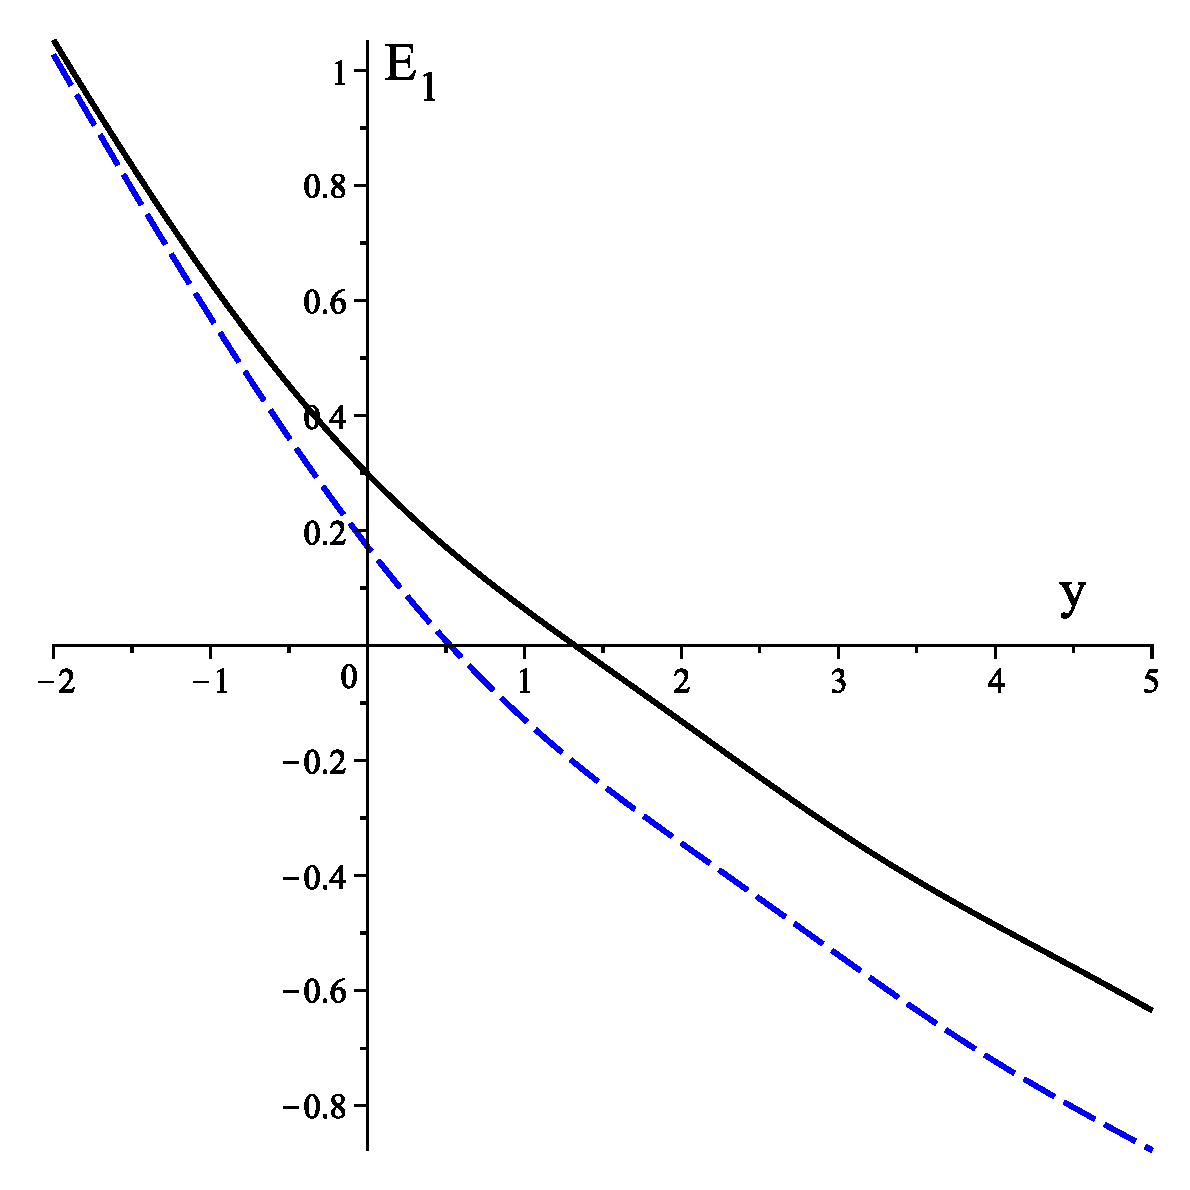
\includegraphics[width=0.45\textwidth,angle=0]{E1_vs_y2}
		\hfill
		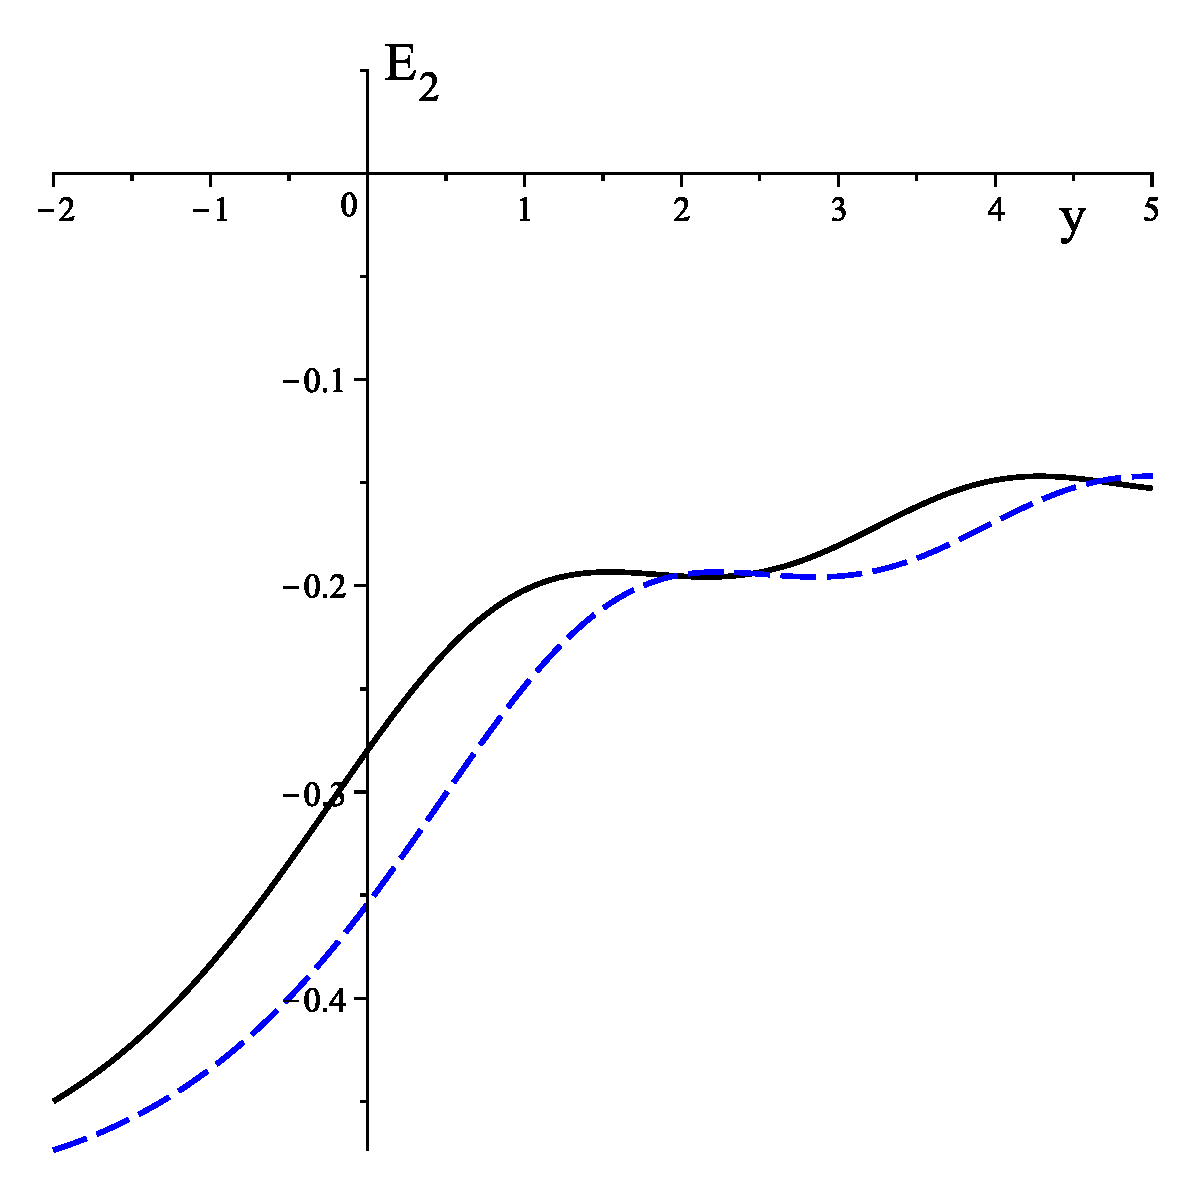
\includegraphics[width=0.45\textwidth,angle=0]{E2_vs_y}
		\\
		%\captionsetup{width=0.5\textwidth}
		\parbox{0.45\textwidth}{\caption{\label{fig:E1_vs_y} Quantity $E_1(y,p,\mu)$ as a function of $y$ at $p=2.0$ ($T^*=0.5$) and $\beta\mu=-2.0$ ($\mu^*=-1.0$) for two different values of $v^*$: Solid line (black): $v^* = 10$, Dash line (blue): $v^* = 5$.}}
		\hfill
		%\captionsetup{width=0.5\textwidth}
		\parbox{0.45\textwidth}{\caption{\label{fig:E2_vs_y} Quantity $E_2(y,p,\mu)$ as a function of $y$ at $p=2.0$ ($T^*=0.5$) and $\beta\mu=-2.0$ ($\mu^*=-1.0$) for two different values of $v^*$: Solid line (black): $v^* = 10$, Dash line (blue): $v^* = 5$.}}
	\end{figure}
	
	As $K_0$, $K_1$, and $p$ all take on strictly positive values, the solution $\bar{y}$ to equation~\eqref{eq:bar_y} is also strictly positive.
	Typical behavior of $E_1(y,p,\mu)$ as a function of $y$ in the single-phase domain is illustrated in Fig.~\ref{fig:E1_vs_y}.
	
	\textbf{Definition}. We say that $(p, \mu)$ belongs to a single-phase domain if $E(y,p,\mu)$ has a unique global maximum $\bar{y} \in \mathbb{R}$ such that
	\begin{equation}
		\label{def:E2}
		E_2(\bar{y}, p, \mu) := \frac{\partial^2}{\partial y^2} E(y,p,\mu)\big|_{y=\bar{y}} < 0.
	\end{equation}
	An explicit expression for $E_2(y,p,\mu)$ reads (cf.~\cite[(20)]{KD22})
	\begin{equation}
		E_2(y,p,\mu) = -\frac{1}{p} + \frac{K_2(y,p,\mu) K(y,p,\mu) - [K_1(y,p,\mu)]^2}{[K_0(y,p,\mu)]^2},
	\end{equation}
	where
	\begin{equation}
		K_2(y,p,\mu) := \frac{\partial}{\partial y} K_1(y,p,\mu) = \sum_{n=0}^{\infty} \frac{n^2 (v^*)^n}{n!} \exp[(y+\beta\mu)n - \frac{ap}{2}n^2].
	\end{equation}
	Typical behavior of $E_2(y,p,\mu)$ as a function of $y$ in the single-phase domain is illustrated in Fig.~\ref{fig:E2_vs_y}.
	
	\begin{mdframed}[linecolor=black,linewidth=1pt,leftline=true]
		In reduced quantities, $E_2$ takes on the form
		\begin{equation}
			\label{def:reducedE2}
			E_2(y,T^*,\mu^*) = -T^* + \frac{K_2(y,T^*,\mu^*) K_0(y,T^*,\mu^*) - [K_1(y,T^*,\mu^*)]^2}{[K_0(y,T^*,\mu^*)]^2},
		\end{equation}
		where
		\begin{equation}
			K_2(y,T^*,\mu^*) = \sum_{n=0}^{\infty} \frac{n^2 (v^*)^n}{n!} \exp[\left(y+\frac{\mu^*}{T^*}\right)n - \frac{a}{2T^*}n^2].
		\end{equation}
	\end{mdframed}
	
	\textbf{Laplace's method.} We apply the Laplace's method~\cite[(1.21)]{Fedoryuk89} to~\eqref{eq:XiInty} and arrive at~(cf.~\cite[(19)]{KD22})
	\begin{equation}
		\Xi(p,\mu) = [-p E_2(\bar{y},p,\mu)]^{-1/2} \exp[N_v E(\bar{y},p,\mu)].
	\end{equation}
	Substituting this into~\eqref{def:eos}, one gets
	\begin{equation}
		P V = k_{\rm B}T \left[-\frac{1}{2} \ln(-p E_2(\bar{y},p,\mu)) + N_v E(\bar{y},p,\mu)\right].
	\end{equation}
	The first term in the square brackets in the right-hand side of the last equation can be neglected in the limit of large $N_v$, and we arrive at (cf.~\cite[(2.27)]{KKD20})
	\begin{equation}
		P v \beta = E(\bar{y},p,\mu),
	\end{equation}
	or
	\begin{equation}
		\label{eos:reduced}
		P^* = T^* E(\bar{y},T^*,\mu^*).
	\end{equation}
	We have obtained an expression for the pressure $P$ as a function of temperature $T$ (through variable $p$) and chemical potential $\mu$, $P = P(T, \mu)$. (We remember that the quantity $\bar{y}$, which is selected from the condition to maximize $E$ at given $T$ and $\mu$, is a function of $T$ and $\mu$, $\bar{y} = \bar{y}(p,\mu)$). The problem here is that we cannot get the solution to~\eqref{eq:bar_y} in an analytic form. Still we can get some results numerically and obtain graphics.
	
	%\pagebreak
	\section{Implicit function theorem}
	The equation~\eqref{eq:bary2} implicitly defines $\bar{y}$ as a function of temperature and chemical potential. We can benefit from the implicit function theorem to get some results for $\bar{y}$ and its derivatives with respect to chemical potential and temperature.
	
	First, let us recall that if a line is given by 
	\begin{equation*}
		{\cal F}(x,y) = 0,
	\end{equation*}
	and if ${\cal F}(x,y)$ is continuously differentiable on some open domain around $(x_0,y_0)$, then
	\begin{equation}
		\frac{{\rm d} y}{{\rm d} x} = - \frac{\partial {\cal F} / \partial x}{\partial {\cal F} / \partial y}.
	\end{equation}
	Applying this to~\eqref{eq:bary2}, we get
	\begin{equation}
		\frac{\partial \bar{y}}{\partial \mu^*} = - \frac{\partial E_1 / \partial \mu^*}{\partial E_1 / \partial \bar{y}}.
	\end{equation}
	By definition~\eqref{def:E2}
	\begin{equation}
		\frac{\partial E_1}{\partial \bar{y}} = E_2.
	\end{equation}
	For $\partial E_1 / \partial \mu^*$ one has
	\begin{equation}
		\frac{\partial E_1}{\partial \mu^*} = \frac{1}{T^*} (E_2 + T^*).
	\end{equation}
	The quantity $E_2(y,T^*,\mu^*)$ can be rewritten as (cf.~\cite[(2.23)]{KKD20})
	\begin{eqnarray}
		E_2(y,T^*,\mu^*) & = & -T^* + \frac{1}{2 [K_0(y,T^*,\mu^*)]^2}
		\\
		& \times & \sum_{n_1, n_2 = 0}^{\infty} \frac{(v^*)^{n_1+n_2}}{n_1!n_2!}(n_1 - n_2)^2 \exp[\left(y + \frac{\mu^*}{T^*}\right)(n_1 + n_2) - \frac{a}{2T^*}(n_1^2 + n_2^2)],\nonumber
	\end{eqnarray}
	leading to
	\begin{equation}
		E_2 + T^* > 0,
	\end{equation}
	and thus
	\begin{equation}
		\frac{\partial E_1}{\partial \mu^*} > 0.
	\end{equation}
	Substituting the results back into $\partial \bar{y}/\partial \mu^*$, one gets
	\begin{equation}
		\left(\frac{\partial \bar{y}}{\partial \mu^*} \right)_{T^*} = -\frac{E_2 + T^*}{T^* E_2}.
	\end{equation}
	We can also consider $\mu^*$ as a function of $y$ and $T^*$, and get
	\begin{equation}
		\left(\frac{\partial \mu^*}{\partial \bar{y}} \right)_{T^*} = -\frac{T^* E_2}{E_2 + T^*}.
	\end{equation}
	Since the condition of maximum implies $E_2 < 0$, it follows
	\begin{equation}
		\left(\frac{\partial \bar{y}}{\partial \mu^*} \right)_{T^*} > 0.
	\end{equation}
	
	
	\pagebreak
	\section{Average number of particles}
	By thermodynamic formulas for the grand canonical ensemble
	\begin{eqnarray}
		\langle N \rangle & = & -\left(\frac{\partial \Omega}{\partial \mu}\right)_{T,V}
		\nonumber\\
		& = & V \left(\frac{\partial P}{\partial \mu}\right)_T.
	\end{eqnarray}
	For reduced density it follows
	\begin{equation}
		\label{eq:dens}
		\rho^* = v\left(\frac{\partial P}{\partial \mu}\right)_T = \left(\frac{\partial P^*}{\partial \mu^*}\right)_T.
	\end{equation}
	As a result of the differentiation of pressure with respect to chemical potential (see Appendix~\ref{sec:app:dens} for details), one gets
	\begin{eqnarray}
		\label{eq:densK}
		\rho^* &=& \frac{K_1(\bar{y}, p,\mu)}{K_0(\bar{y},p,\mu)} = \frac{K_1(\bar{y},T^*,\mu^*)}{K_0(\bar{y},T^*,\mu^*)}.
	\end{eqnarray}
	
	The quantity $\rho^*$, on the one hand, is the reduced particle number density, which is the notation commonly used in the literature on simple liquids~\cite{HansenMcDonald13}. In the context of the cell model, on the other hand, it also has the meaning of the average number of particles per cell, because
	\begin{equation}
		\rho^* = \frac{\langle N \rangle}{V} v = \frac{\langle N \rangle}{N_v}.
	\end{equation}
	
	From~\eqref{eq:bar_y} it also follows that
	\begin{equation}
		\label{rho_vs_T_mu}
		\rho^*(T,\mu) = \bar{y}(T,\mu) T^*.
	\end{equation}
	%This enables us to calculate the equation of state.
	
	\section{Equation of state}
	We have got relation $P^* = P^*(T^*, \mu^*)$ in~\eqref{eos:reduced}. Now, having found the density $\rho^* = \rho^*(T^*,\mu^*)$ in~\eqref{rho_vs_T_mu}, we can formally solve this equation with respect to $\mu$ to find $\mu^* = \mu^*(T^*,\rho^*)$, and substitute back into~\eqref{eos:reduced} to get pressure as a function of density and temperature (cf.~\cite[(2.28)]{KKD20})
	\begin{equation}
		\label{eos}
		P^* = T^* E\left[\frac{\rho^*}{T^*},T^*, \mu^*(T^*,\rho^*)\right],
	\end{equation}
	which will be the equation of state in convenient, (wide-spread, generally accepted) terms. However, such task is not an easy one, and at the moment we can solve~\eqref{rho_vs_T_mu} with respect to $\mu$ only numerically. Nevertheless, even formal consideration of equation~\eqref{eos} is helpful to determine the critical points coordinates, see the next Section~\ref{sec:CP}.
	
	\pagebreak
	\section{\label{sec:CP} Critical point coordinates}
	From the general theories of phase transitions and critical phenomena, we have got a recipe to find the coordinates of the critical point from an equation of state in the form $P=P(T,\rho)$. Since the critical point is the inflection point on the critical isotherm, we have two conditions
	\begin{equation}
		\begin{split}
			\left(\frac{\partial P^*}{\partial \rho^*}\right)_{T^*} = 0;
			\\
			\left(\frac{\partial^2 P^*}{\partial (\rho^*)^2}\right)_{T^*} = 0.
		\end{split}		
	\end{equation}
	As is shown in Appendix~\ref{sec:app:cp}, these two conditions are equivalent to
	\begin{equation}
		\begin{split}
			E_2 = 0,
			\\
			E_3 = 0,
		\end{split}
	\end{equation}
	where
	\begin{equation}
		\begin{split}
			E_3 &:= \frac{\partial^3}{\partial y^3} E(T,\mu; y)\big|_{y=\bar{y}} 
			\\
			& = \frac{\partial}{\partial \bar{y}} E(T,\mu; \bar{y})
			\\
			& = \frac{K_3}{K_0} - \frac{3 K_2 K_1}{K_0^2} + \frac{2K_1^3}{K_0^3}.
		\end{split}
	\end{equation}
	Together with Eq.~\eqref{eq:bar_y} we have three equations with three unknown values for $T^*$, $\mu^*$, and $\bar{y}$:
	\begin{equation}
		\label{eq:system}
		\begin{cases}
			E_1(T^*,\mu^*; \bar{y}) = 0,\\
			E_2(T^*,\mu^*; \bar{y}) = 0,\\
			E_3(T^*,\mu^*; \bar{y}) = 0.
		\end{cases}
	\end{equation}
	We can resolve this system of equations numerically, and find the critical point coordinates $T^*_c$, $\mu^*_c$, and $\bar{y}_c$.
	
	The cell model with Curie-Weiss interaction is known to possess multiple critical points~\cite{KKD18,KKD20,KD22}. Thus the system of equations~\eqref{eq:system} has many sets of solutions. We denote such solutions by natural numbers $n$, starting with $n=1$ for the lowest critical temperature. Table~\ref{tab:cp} contains the found sets of solutions, as well as other physical quantities values at the critical points calculated based on $T^*_c$, $\mu^*_c$, and $\bar{y}_c$.
	
	\begin{table}[h]
		\centering
		\caption{The critical point values for some quantities. The number $n$ denotes the critical points starting with $n=1$ for the one with the lowest temperature.}
		\begin{tabular}{|c|c|c|c|c|c|c|}
			\hline
			$n$ & $T^*_c$ & $\mu^*_c$ & $\bar{y}_c$ & $\beta^*_c$ (or $p_c$) & $\rho^*_c$ & $P^*_c$ \\
			\hline
			1 & 0.254567 & -0.313065 & 2.01870 & 3.92823 & 0.513896 & 0.0503397  \\
			2 & 0.261881 & 0.0587688 & 5.74906 & 3.81852 & 1.50557 & 0.437695  \\
			3 & 0.265254 & 0.363828 & 9.43632 & 3.76996 & 2.50303 & 1.05817 \\
			4 & \textcolor{blue}{0.267242} & \textcolor{blue}{0.639949} & \textcolor{blue}{13.1039} & \textcolor{blue}{3.74193} & \textcolor{blue}{3.50191} & \textcolor{blue}{1.89369} \\
			5 & & & & & & \\
			\hline
			$n$ & $\beta_c\mu_c$ & $\beta_c P_c v$ & $\bar{z}_c=\bar{y}_c+\mu^*_c/T^*_c$ & $\bar{y}_c+\mu^*_c/T^*_c + \ln v^*$ & $S^*_c$ & \\
			\hline
			1 & -1.22979 & 0.197746 & 0.788910 & 2.39835 & 4.48401 & \\
			2 & 0.224410 & 1.67135 & 5.97347 & 7.58291 & 3.35912 & \\
			3 & 1.37162 & 3.98927 & 10.8079 & 12.4174 & 2.90550 & \\
			4 & \textcolor{blue}{2.39464}  & \textcolor{blue}{7.08603}& \textcolor{blue}{15.4985} & \textcolor{blue}{17.1080} & & \\
			5 &  & & & & & \\
			\hline
		\end{tabular}
		\label{tab:cp}
	\end{table}
	
	\pagebreak
	\section{Entropy}
	By thermodynamic formulas for the grand canonical ensemble
	\begin{equation}
		S = -\left(\frac{\partial \Omega}{\partial T}\right)_{V,\mu} = V\left(\frac{\partial P}{\partial T}\right)_{\mu}
	\end{equation}
	where $\Omega = -k_{\rm B}T \ln \Xi$ is the grand potential. 
	
	Now, there are two possibilities to normalize entropy. One possibility is to normalize it by the average number of particles
	\begin{equation}
		S^{*} = \frac{S}{k_{\rm B} \langle N \rangle},
	\end{equation}
	and call this quantity the entropy per particle. Another possibility is to normalize it by the number of cells
	\begin{equation}
		S^{**} = \frac{S}{k_{\rm B}N_v},
	\end{equation}
	and call this quantity the entropy per cell. The usage of the entropy per particle, $S^*$, is more common in the theory of many-particle systems~\cite{HansenMcDonald13}, while the entropy per cell, $S^{**}$, may be useful in cell (or lattice) models. For completeness, we will present results for both quantities. We will also call $S^*$ the reduced entropy.
	
	
	The reduced entropy reads
	\begin{eqnarray}
		S^* & = & \frac{v}{k_{\rm B}} \frac{N_v}{\langle N \rangle} \left(\frac{\partial P}{\partial T}\right)_{\mu}
		\\
		& = & \frac{1}{\rho^*}\left(\frac{\partial P^*}{\partial T^*}\right)_{\mu}
		\\
		& = & \frac{(\partial P^* / \partial T^*)_{\mu}}{(\partial P^* / \partial \mu^*)_T}.
	\end{eqnarray}
	By~\eqref{eos:reduced}
	\begin{equation}
		\label{eq:entropy}
		S^* = \frac{1}{\rho^*} 
		\left[ 
		E(\bar{y},T^*,\mu^*) + T^* \left(\frac{\partial E(\bar{y},T^*,\mu^*)}{\partial T^*}\right)_{\mu} 
		\right].
	\end{equation}
	The result of calculation is
	\begin{equation}
		S^* = \left(\frac{3}{2} - \beta\mu\right) -p \frac{K_1}{K_0} + \frac{K_0 \ln K_0}{K_1} + \frac{ap}{2} \frac{K_2}{K_1},
	\end{equation}
	or in the reduced quantities
	\begin{equation}
		\label{S_vs_T_mu}
		S^* = \left(\frac{3}{2} - \frac{\mu^*}{T^*}\right) - \frac{1}{T^*}\frac{K_1}{K_0} + \frac{K_0 \ln K_0}{K_1} + \frac{a}{2T^*} \frac{K_2}{K_1}.
	\end{equation}
	The first contribution to the entropy corresponds to the entropy of non-interacting molecules in a lattice, or an ideal lattice gas contribution, see~\cite[(47.4)]{Hill56}, if we account for the ideal-gas chemical potential $\mu_{\rm id} = k_{\rm B}T \ln(N\Lambda^3/V)$. 
	
	
	\textbf{Entropy per cell.} The relation between $S^*$ and $S^{**}$ is
	\begin{equation}
		S^* = \frac{1}{\rho^*} S^{**},
	\end{equation}
	where
	\begin{equation}
		\label{eq:entropy2}
		S^{**}  = \left(\frac{\partial P^*}{\partial T^*}\right)_{\mu}.
	\end{equation}
	The expressions for the entropy per cell is
	\begin{equation}
		S^{**} = -\frac{\bar{y}^2}{p} + \ln K_0(\bar{y},p,\mu) + \frac{\left[\left(\frac{3}{2} - \beta\mu\right)K_1(\bar{y},p,\mu) + \frac{ap}{2}K_2(\bar{y},p,\mu) \right]}{K_0(\bar{y},p,\mu)}
	\end{equation}
	or in reduced quantities
	\begin{eqnarray}
		S^{**} & = & -T^* \bar{y}^2 + \ln K_0(\bar{y},T^*,\mu^*) + \left[\left(\frac{3}{2} - \frac{\mu^*}{T^*}\right) K_1(\bar{y},T^*,\mu^*) + \frac{a}{2T^*} K_2(\bar{y},T^*,\mu^*) \right] [K_0(\bar{y},T^*,\mu^*)]^{-1}
		\nonumber \\
		& = & -T^* \bar{y}^2 + \ln K_0 + \frac{1}{K_0}\left[\left(\frac{3}{2} - \frac{\mu^*}{T^*}\right) K_1 + \frac{a}{2T^*} K_2 \right]
	\end{eqnarray}
	Details or calculation are present in Appendix~\ref{sec:app:entropy}.
	
	\begin{figure}[htbp]
		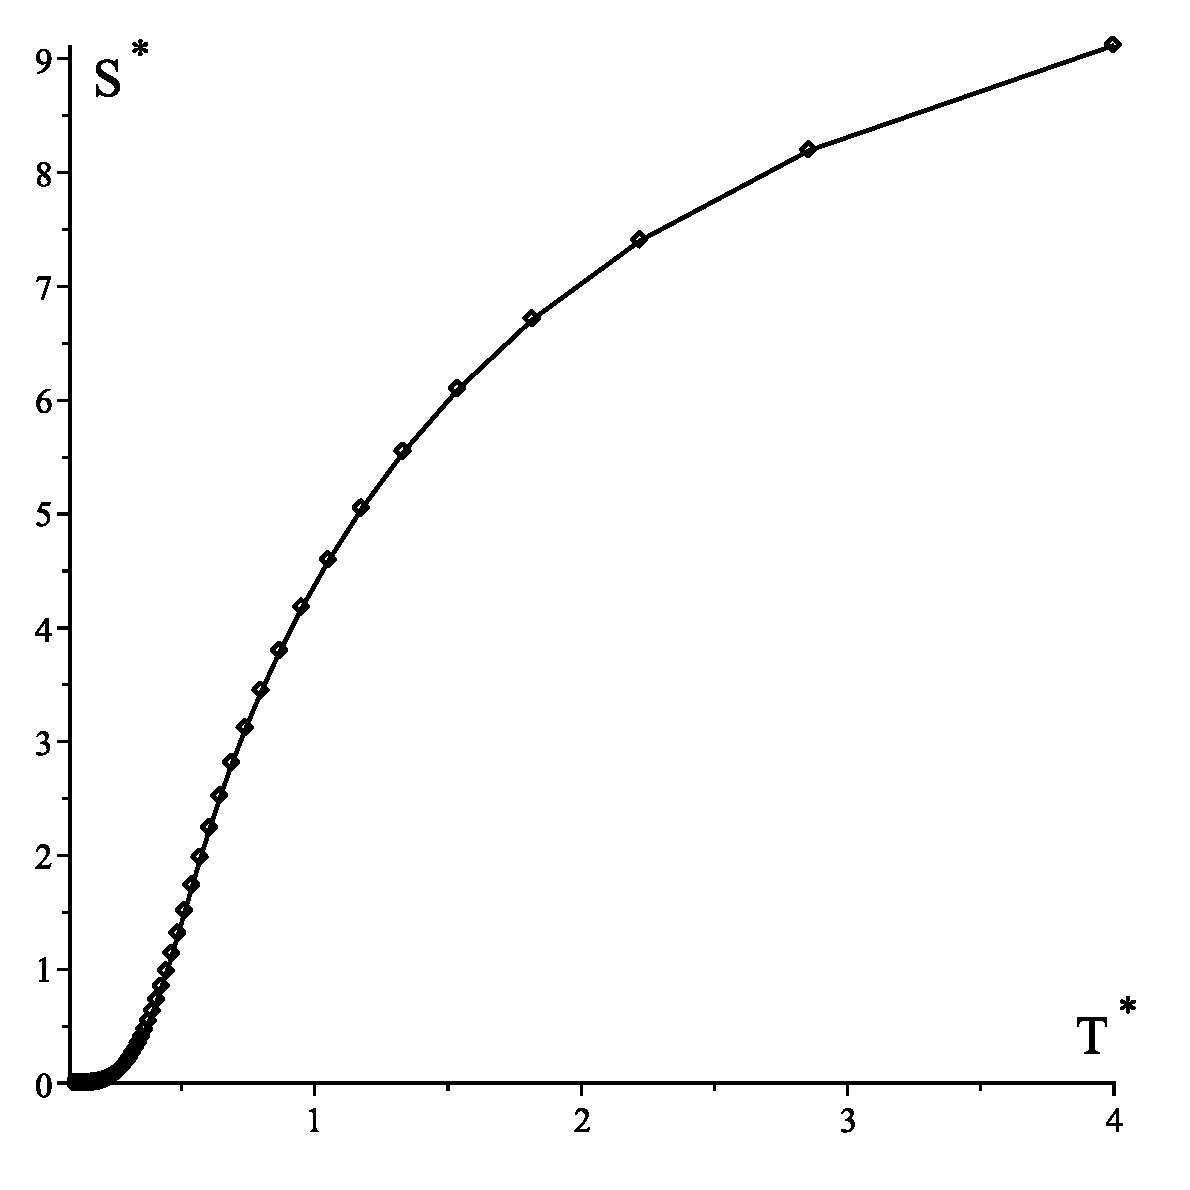
\includegraphics[width=0.55\textwidth,angle=0]{S_vs_T1}
		\centering
		%\hfill
		%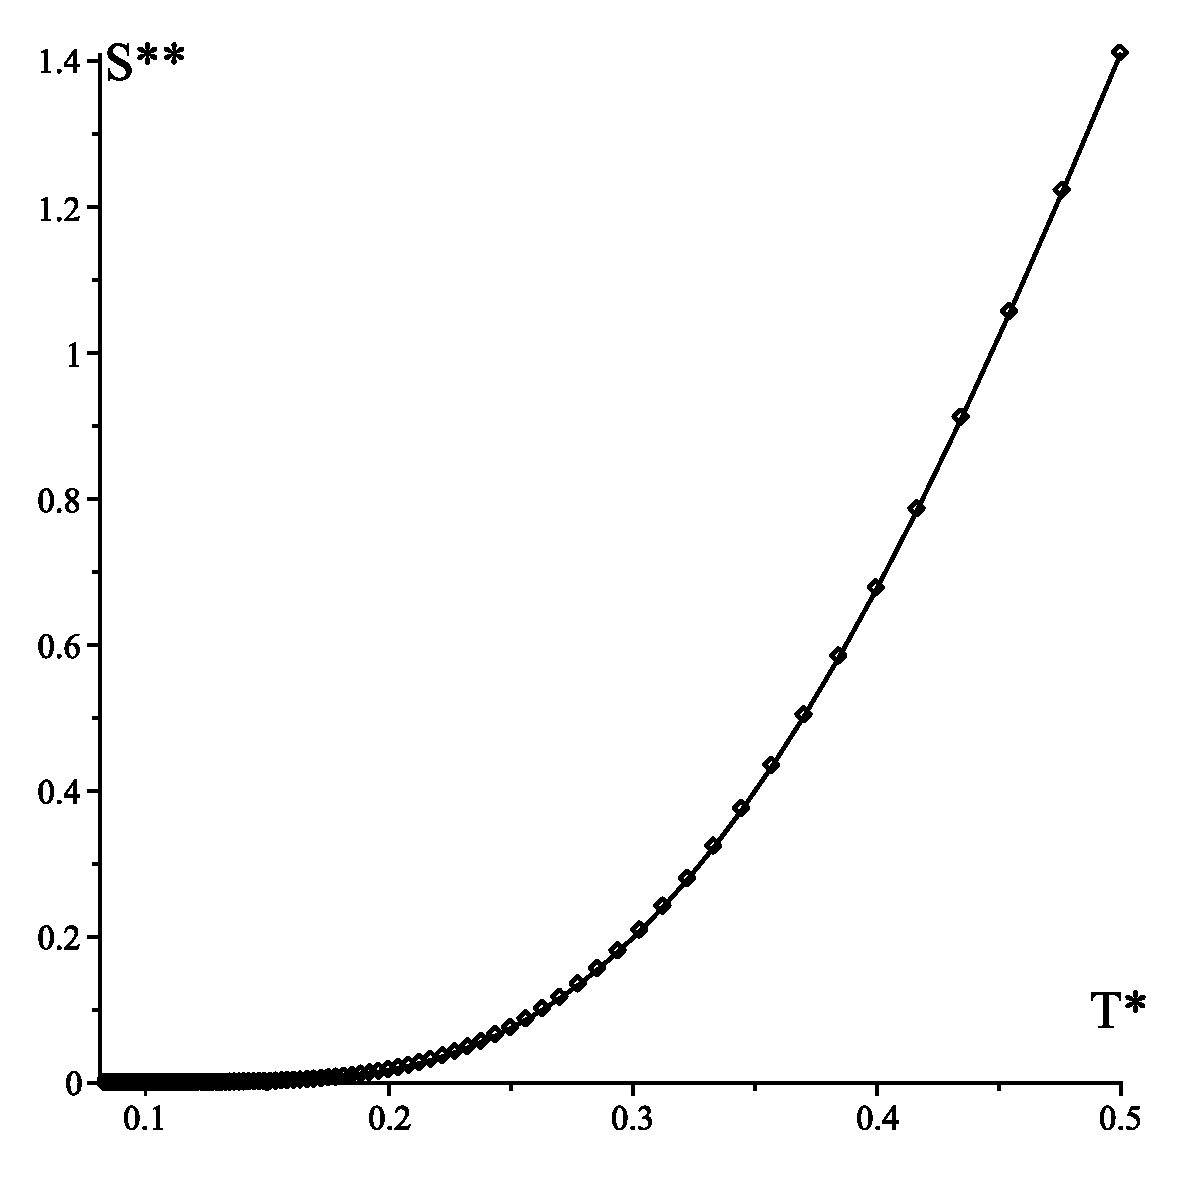
\includegraphics[width=0.45\textwidth,angle=0]{SS_vs_T2}
		%\\
		\captionsetup{width=0.5\textwidth}
		%\parbox{0.45\textwidth}
		{\caption{\label{fig:S_vs_T1} Entropy $S^{*}(\bar{y},T^*,\mu^*)$ as a function of $T^*$ at $\mu^*=-1.0$ ($v^* = 5$).}}
		%\hfill
		%\captionsetup{width=0.5\textwidth}
		%\parbox{0.45\textwidth}{\caption{\label{fig:S_vs_T2} Entropy $S^{**}(\bar{y},T^*,\mu^*)$ as a function of $T^*$ at $\mu^*=-1.0$ ($v^* = 5$)}}
	\end{figure}
	
	\begin{figure}[htbp]
		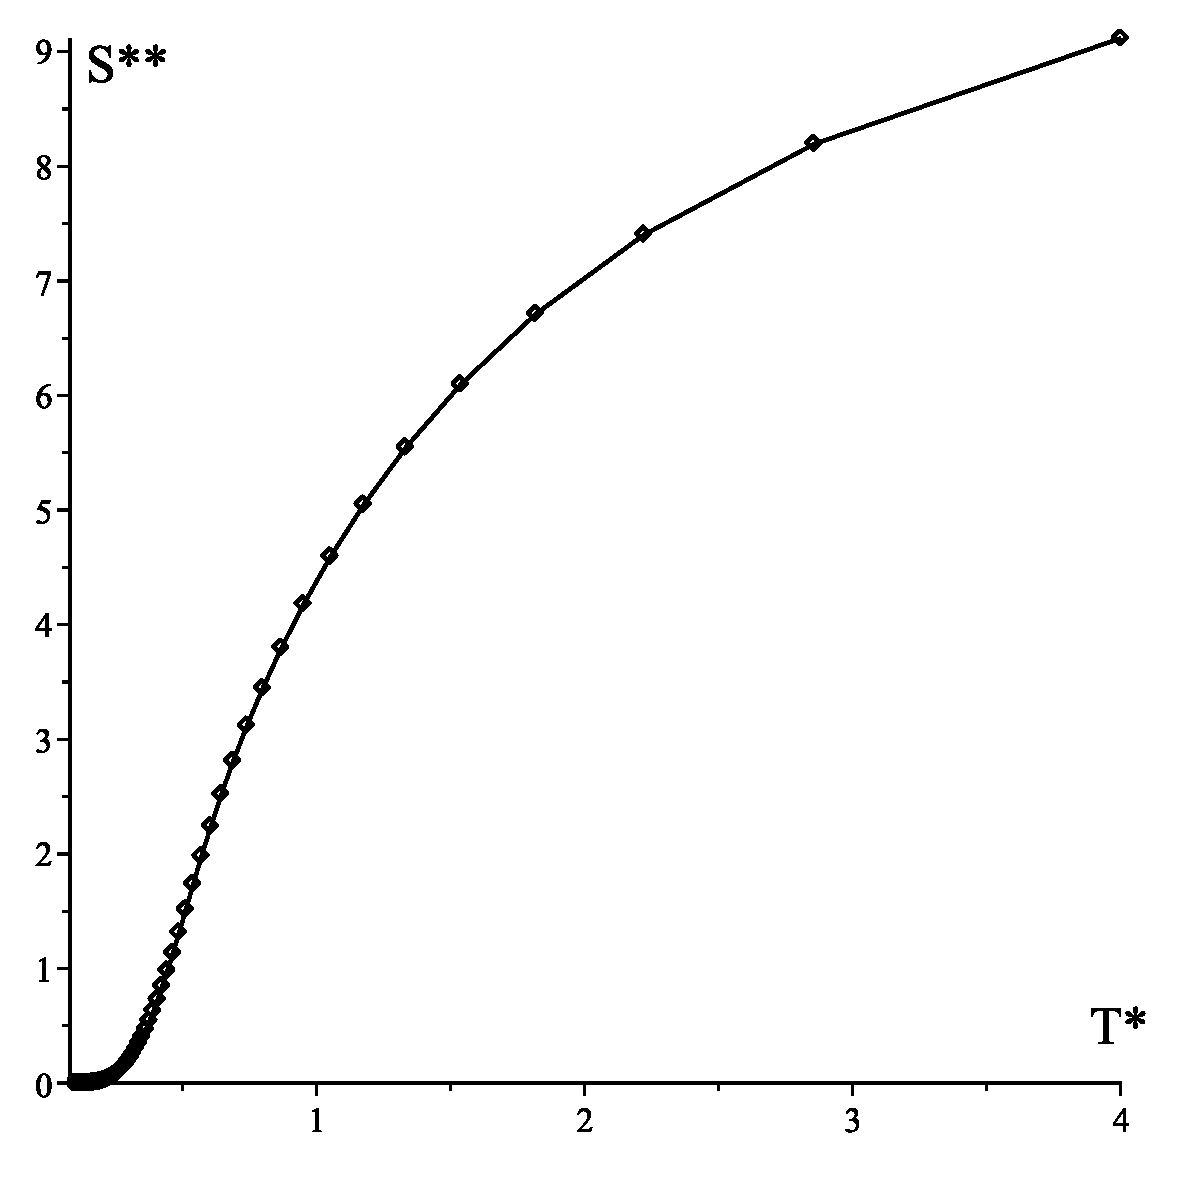
\includegraphics[width=0.45\textwidth,angle=0]{SS_vs_T1}
		\hfill
		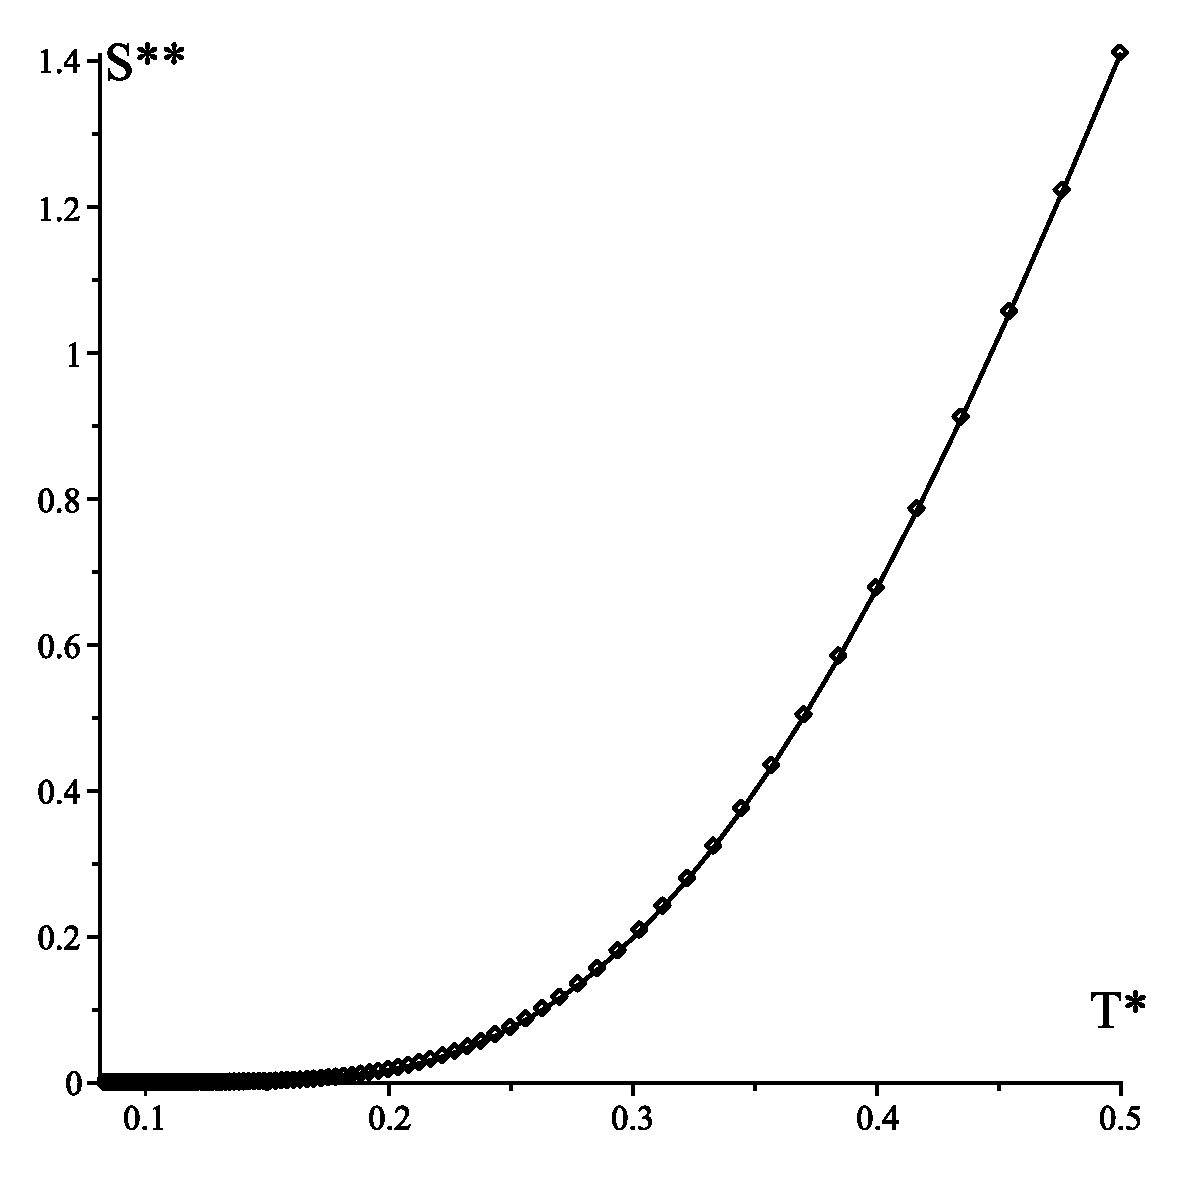
\includegraphics[width=0.45\textwidth,angle=0]{SS_vs_T2}
		\\
		%\captionsetup{width=0.5\textwidth}
		\parbox{0.45\textwidth}{\caption{\label{fig:SS_vs_T1} Entropy $S^{**}(\bar{y},T^*,\mu^*)$ as a function of $T^*$ at $\mu^*=-1.0$ ($v^* = 5$).}}
		\hfill
		%\captionsetup{width=0.5\textwidth}
		\parbox{0.45\textwidth}{\caption{\label{fig:SS_vs_T2} Entropy $S^{**}(\bar{y},T^*,\mu^*)$ as a function of $T^*$ at $\mu^*=-1.0$ ($v^* = 5$).}}
	\end{figure}
	
	\textbf{Graphics for Entropy.} The dependence of the reduced entropy $S^*$ on temperature $T^*$ at a given chemical potential is illustrated in Fig.~\ref{fig:S_vs_T1}. Figures~\ref{fig:SS_vs_T1} and~\ref{fig:SS_vs_T2} illustrate the dependence of entropy per cell $S^{**}$ on temperature $T^*$ at a constant chemical potential. The two figures for $S^{**}$ show the same functional dependency but focus on different temperature ranges.
	
	\begin{figure}[htbp]
		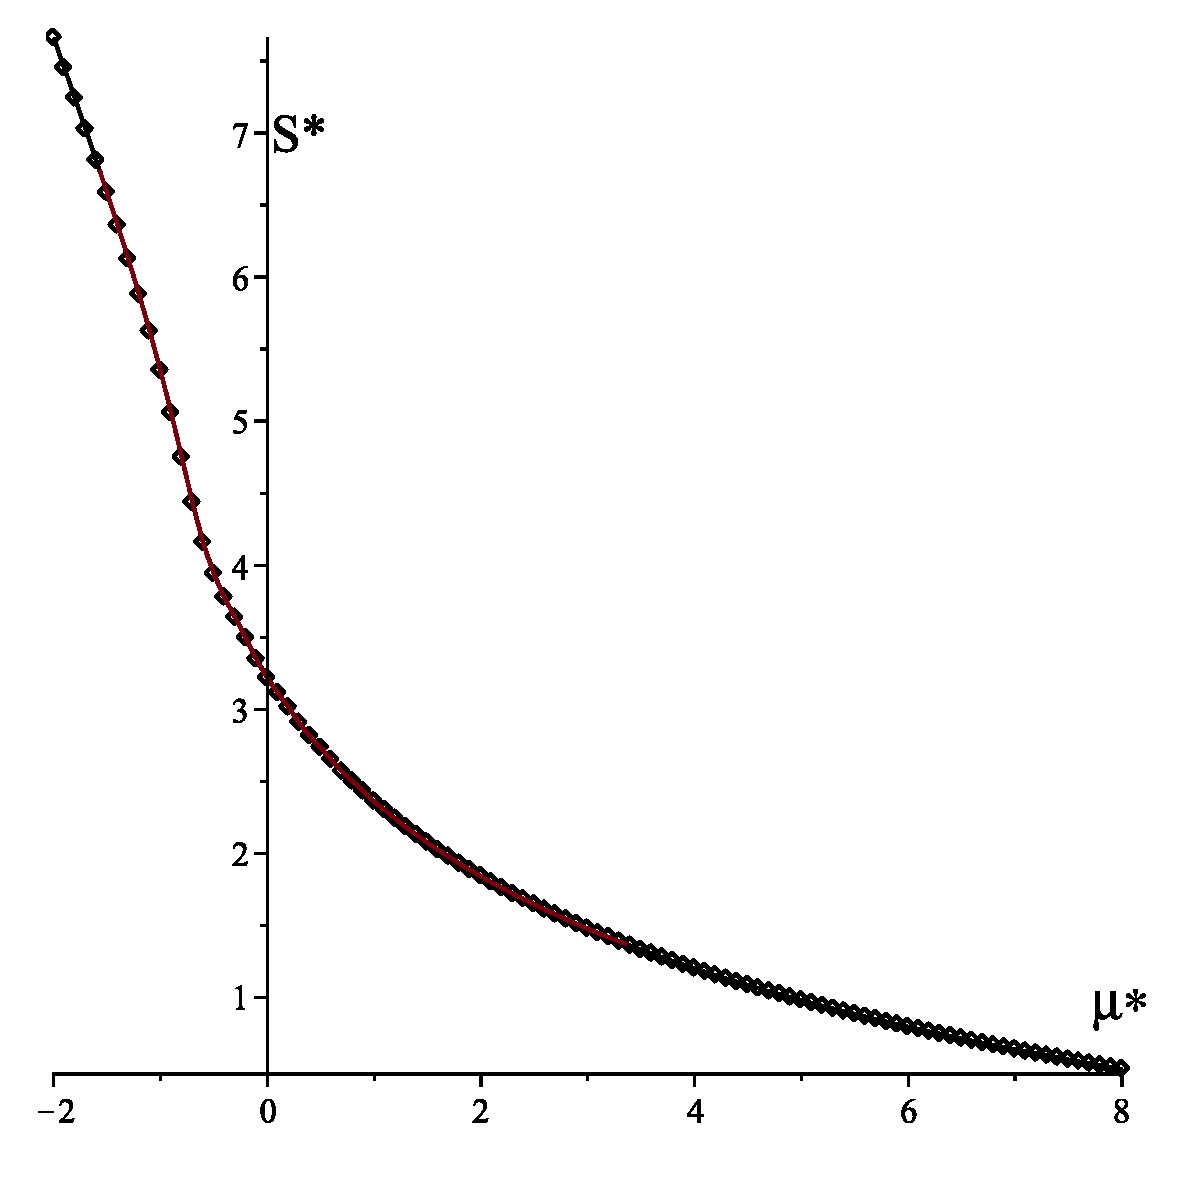
\includegraphics[width=0.45\textwidth,angle=0]{S_vs_mu}
		\hfill
		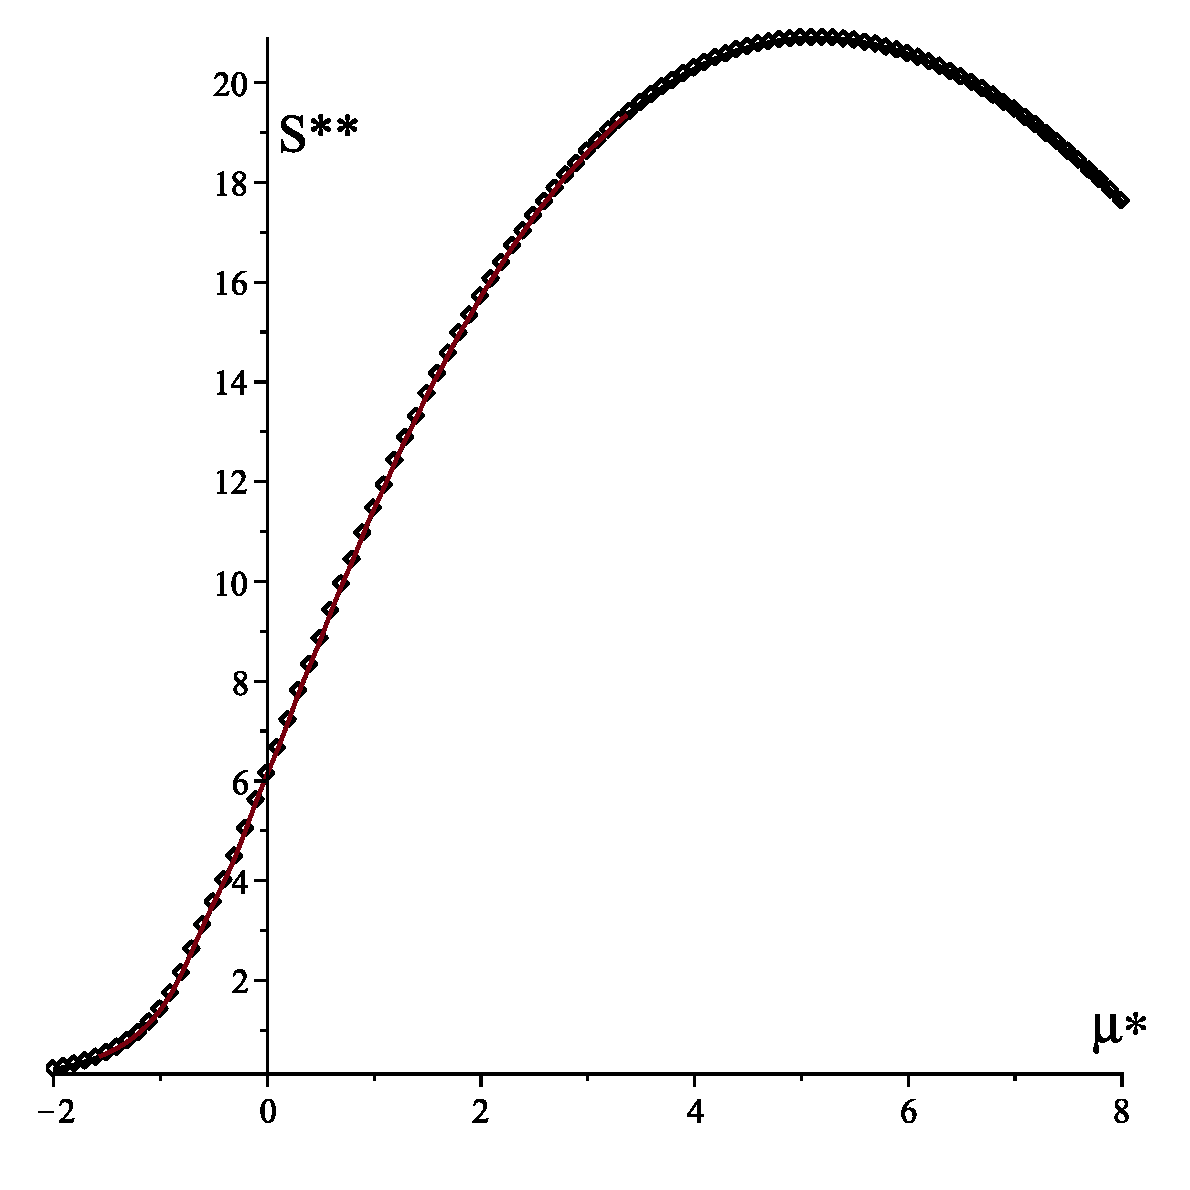
\includegraphics[width=0.45\textwidth,angle=0]{SS_vs_mu}
		\\
		%\captionsetup{width=0.5\textwidth}
		\parbox{0.45\textwidth}{\caption{\label{fig:S_vs_mu} Entropy per particle $S^{*}(\bar{y},T^*,\mu^*)$ as a function of $\mu^*$ at $T^*=0.5$ ($v^* = 5$).}}
		\hfill
		%\captionsetup{width=0.5\textwidth}
		\parbox{0.45\textwidth}{\caption{\label{fig:SS_vs_mu} Entropy per cell $S^{**}(\bar{y},T^*,\mu^*)$ as a function of $\mu^*$ at $T^*=0.5$ ($v^* = 5$).}}
	\end{figure}
	
	The dependence of the reduced entropy $S^*$ on chemical potential $\mu^*$ at a given temperature is illustrated in Fig.~\ref{fig:S_vs_mu}. That of $S^{**}$ is shown in Fig.~\ref{fig:SS_vs_mu}.
	
	\begin{figure}[htbp]
		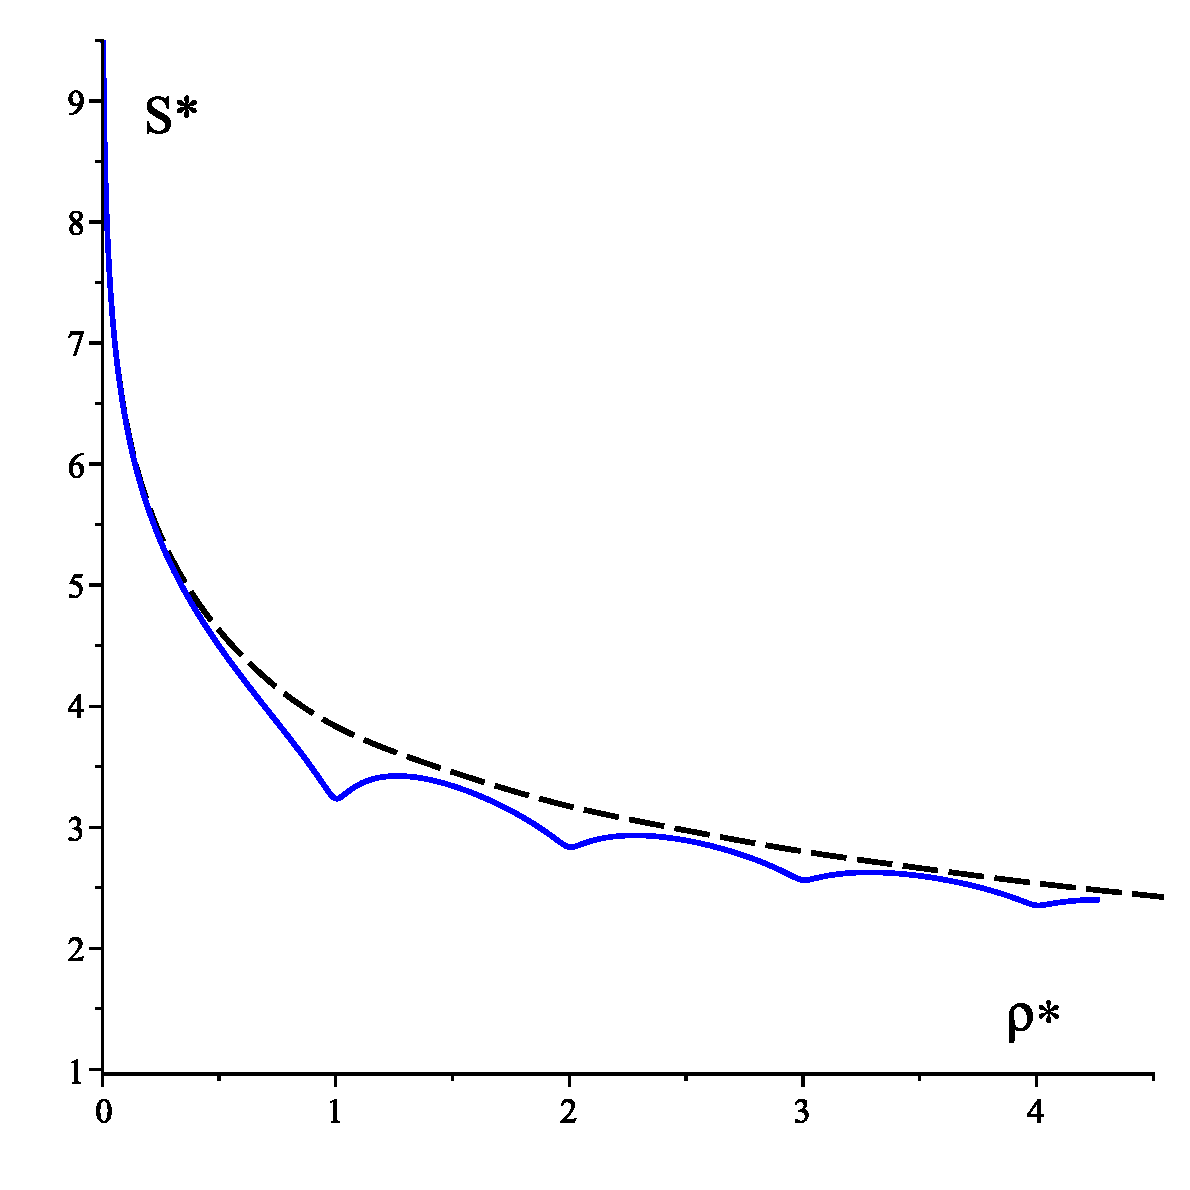
\includegraphics[width=0.45\textwidth,angle=0]{S_vs_rho}
		\hfill
		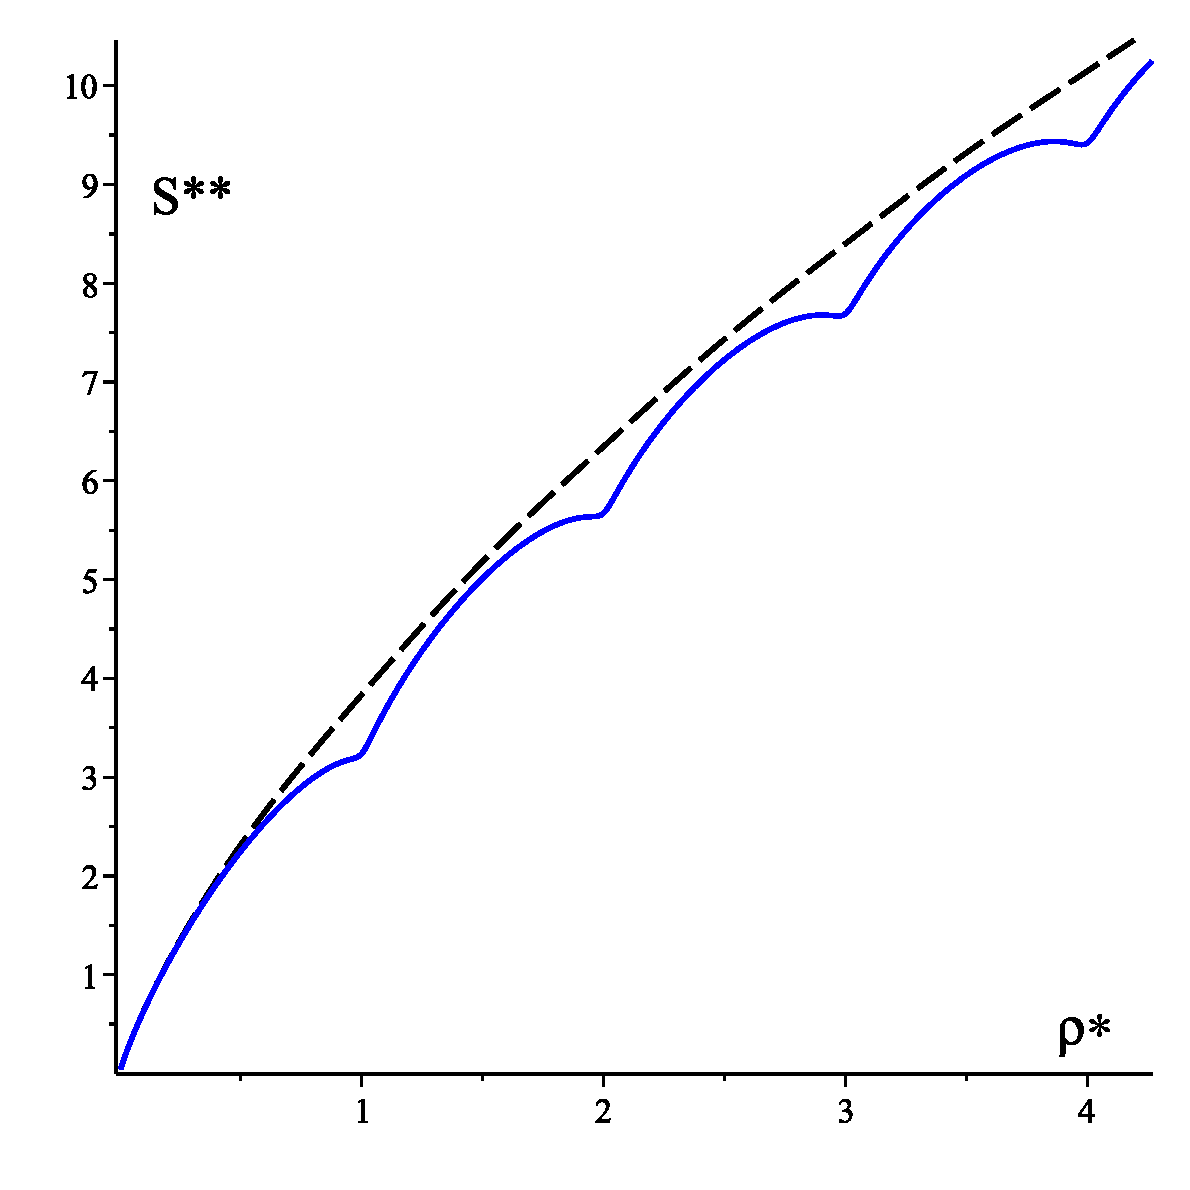
\includegraphics[width=0.45\textwidth,angle=0]{SS_vs_rho}
		\\
		%\captionsetup{width=0.5\textwidth}
		\parbox{0.45\textwidth}{\caption{\label{fig:S_vs_rho} Entropy per particle $S^{*}$ as a function of $\rho^*$, (Dashed black line) at $T^*=0.5$, and (Solid blue line) at $T^*=0.15$.}}
		\hfill
		%\captionsetup{width=0.5\textwidth}
		\parbox{0.45\textwidth}{\caption{\label{fig:SS_vs_rho} Entropy per cell $S^{**}$ as a function of $\rho^*$, (Dashed black line) at $T^*=0.5$, and (Solid blue line) at $T^*=0.15$.}}
	\end{figure}
	
	The equation for entropy~\eqref{S_vs_T_mu} expresses entropy as a function of temperature and chemical potential. If we want to have entropy as a function of temperature and density, we combine equations~\eqref{S_vs_T_mu} and~\eqref{rho_vs_T_mu} into a parametric equation for entropy, with $\mu$ being the parameter. This way we can plot the dependence of entropy on density at a given temperature. Such dependencies are present in Fig.~\ref{fig:S_vs_rho} and~Fig.~\ref{fig:SS_vs_rho}.
	

	\pagebreak
	\section{The special function $K_0$ and its integral representation}
	
	\be\label{KOZ}
	K_0(z)=\sum_{n\ge0}\frac1{n!}\,\e^{zn-an^2}
	\ee
	Note that sum in \eqref{KOZ} is precisely of the same functional form as that in the definition \eqref{ZGR} of the grand partition function up to replacements
	\be
	N\to n,\qquad z\to\e^{-z},\MM{and}Z_n\to\e^{-an^2}.
	\ee
	
	The integral representation of $K_0(z)$ is given by
	\be\label{KOI}
	K_0(z)=\frac1{2\sqrt\pi}\int_{-\infty}^\infty {\rm d}x \e^{-\frac{x^2}4}
	\mbox{exp}\left(\e^{z+ix\sqrt a}\right),
	\ee
	or, in the form of a manifestly real integral,
	\be\label{KOR}
	K_0(z)=\frac1{2\sqrt\pi}\int_{-\infty}^\infty {\rm d}x \e^{-\frac{x^2}4}
	\mbox{exp}\left[\e^z\cos(x\sqrt a\,)\right]
	\cos\left[\e^z\sin(x\sqrt a\,)\right].
	\ee
	
	Can you calculate the asymptotic behavior as $z\to+\infty$ of two last integrals?
	
	I have succeeded to calculate the leading $z\to+\infty$ asymptotics only for two integrals
	\be
	K_0^{(a)}(z) = \frac1{2\sqrt\pi} \int_{-\infty}^\infty {\rm d}x \e^{-\frac{x^2}4}
	\mbox{exp}\left[\e^z\cos(x\sqrt a\,)\right]\qquad\mbox{and}\qquad
	\ee
	\be
	K_0^{(b)}(z) = \frac1{2\sqrt\pi} \int_{-\infty}^\infty {\rm d}x \e^{-\frac{x^2}4}
	\cos\left[\e^z\sin(x\sqrt a\,)\right]
	\ee
	resulting from \eqref{KOR} by deleting one of the last two factors.
	
	The leading asymptotics are the following
	\begin{equation}
		K_0^{(a)}(z) \sim \frac{\exp({\rm e}^z)}{\sqrt{2 {\rm e}^z}}, \quad \text{as } z \to +\infty
	\end{equation}
	and
	\begin{equation}
		K_0^{(b)}(z) \sim \sqrt{\frac{2}{\pi {\rm e}^z}} \cos({\rm e}^z - \pi/4), \quad \text{as } z \to +\infty.
	\end{equation}
	
	
	\appendix
	
	\pagebreak
	
	\section{\label{sec:app1} Explicit derivation of $E(y,p,\mu)$ and $K(y,p,\mu)$}
	In this appendix, the explicit transformations through Eqs.~(2.11)--(2.15) is presented. Substituting the Gaussian integral~\eqref{eq:gaussInt} into~\eqref{eq:XiPi}, one proceeds as follows
	\begin{eqnarray}
		\Xi 
		&=& 
		\sum_{\varrho \in \mathbb{N}_0^{N_v}} \sqrt{\frac{N_v}{2\pi p}} \int\limits_{-\infty}^{\infty} \exp(-N_v \frac{y^2}{2p}) 
		\prod\limits_{l=1}^{N_v} \frac{(v^*)^{\varrho_l}}{\varrho_l !} 
		\exp[(y + \beta\mu) \varrho_l - \frac{ap}{2}\varrho_l^2] {\rm d}y
		\nonumber\\
		&=&
		\sqrt{\frac{N_v}{2\pi p}} \sum_{\varrho_1=0}^{\infty} \ldots \sum_{\varrho_{N_v}=0}^{\infty} 
		\int\limits_{-\infty}^{\infty} {\rm e}^{-N_v \frac{y^2}{2p}} 
		\prod\limits_{l=1}^{N_v} \frac{(v^*)^{\varrho_l}}{\varrho_l !} 
		\exp[(y + \beta\mu) \varrho_l - \frac{ap}{2}\varrho_l^2] {\rm d}y
		\nonumber\\
		&=&
		\sqrt{\frac{N_v}{2\pi p}} \int\limits_{-\infty}^{\infty} {\rm e}^{-N_v \frac{y^2}{2p}}
		\left\{ 
			\sum_{\varrho_1=0}^{\infty} \frac{(v^*)^{\varrho_1}}{\varrho_1 !} \exp[(y + \beta\mu) \varrho_1 - \frac{ap}{2}\varrho_1^2] 
		\right\}
		\nonumber\\
		&& 
		\times \ldots \times 
		\left\{ 
			\sum_{\varrho_{N_v}=0}^{\infty} \frac{(v^*)^{\varrho_{N_v}}}{\varrho_{N_v} !} \exp[(y + \beta\mu) \varrho_{N_v} - \frac{ap}{2}\varrho_{N_v}^2] 
		\right\}
		{\rm d}y
		\nonumber\\
		&=&
		\sqrt{\frac{N_v}{2\pi p}} \int\limits_{-\infty}^{\infty} {\rm e}^{-N_v \frac{y^2}{2p}}
		\exp( \ln \left\{\sum_{n=0}^{\infty} \frac{(v^*)^{n}}{n!} \exp[(y + \beta\mu)n - \frac{ap}{2}n^2] \right\}^{N_v} ) {\rm d}y
		\nonumber\\
		&=&
		\sqrt{\frac{N_v}{2\pi p}} \int\limits_{-\infty}^{\infty}
		\exp 
		\left\{ N_v 
			\left[ -\frac{y^2}{2p} + 
			\ln(\sum_{n=0}^{\infty} \frac{(v^*)^{n}}{n!} {\rm e}^{(y + \beta\mu)n - \frac{ap}{2}n^2}) 
			\right] 
		\right\} {\rm d}y,
	\end{eqnarray}
	and arrives at Eqs.~\eqref{eq:XiInty}, \eqref{def:E}, and~\eqref{def:K}
	\begin{equation}
		\Xi = \sqrt{\frac{N_v}{2\pi p}} \int\limits_{-\infty}^{\infty}
		\exp 
		\left\{ N_v 
		\left[ -\frac{y^2}{2p} + 
		\ln K(y,p,\mu) 
		\right] 
		\right\}.
	\end{equation}
	
	\pagebreak	
		
	\section{\label{sec:app:dens} Calculation of Density}
	This Appendix contains explicit calculation of density from~\eqref{eq:dens}. By~\eqref{eos:reduced}
	\begin{equation}
		\rho^* = \frac{\partial P^*}{\partial \mu^*} = T^* \frac{\partial E}{\partial \mu^*}.
	\end{equation}
	Then
	\begin{equation}
		\frac{\partial E}{\partial \mu^*} = \frac{1}{K_0} \frac{\partial K_0}{\partial \mu^*}.
	\end{equation}
	By~\eqref{def:K}
	\begin{equation}
		\frac{\partial K_0}{\partial \mu^*} = \frac{1}{T^*}K_1.
	\end{equation}
	Substituting these derivatives back into above formulas, we arrive at
	\begin{equation}
		\frac{\partial E}{\partial \mu^*} = \frac{1}{T^*} \frac{K_1}{K},
	\end{equation}
	and finally
	\begin{equation}
		\left(\frac{\partial P^*}{\partial \mu^*} \right)_T = \frac{K_1}{K_0} = \rho^*.
	\end{equation}
	
	\section{\label{sec:app:cp} System of equations for the critical point coordinates}
	
	
	\section{\label{sec:app:entropy} Calculation of Entropy}
	This Appendix contains explicit calculation of entropy from Eq.~\eqref{eq:entropy} by taking derivatives of pressure with respect to temperature
	\begin{equation}
		S^{*} = \frac{1}{\rho^*} \left[E + T^* \left(\frac{\partial E}{\partial T^*}\right)_{\mu}\right];
	\end{equation}
	\begin{equation}
		E = -\frac{1}{2}T^* \bar{y}^2 + \ln K_0.
	\end{equation}
	\begin{equation}
		\frac{\partial E}{\partial T^*} = -\frac{1}{2}\bar{y}^2 + \frac{1}{K_0}\frac{\partial}{\partial T^*} K_0.
	\end{equation}
	\begin{eqnarray}
		\frac{\partial K_0}{\partial T^*} & = & \sum_{n=0}^{\infty} \frac{n (v^*)^{n-1}}{n!} \exp(F_n) \frac{\partial v^*}{\partial T^*} 
		\nonumber\\
		& + & \sum_{n=0}^{\infty} \frac{(v^*)^n}{n!} \exp(F_n) \frac{\partial}{\partial T^*} F_n,
	\end{eqnarray}
	where we temporary introduced
	\begin{eqnarray*}
		F_n & = & \left(y + \frac{\mu^*}{T^*} \right)n -\frac{a}{2T^*}n^2
		\\
		& = & \left(y + \beta\mu \right)n -\frac{ap}{2}n^2.
	\end{eqnarray*}
	The derivatives of $v^*$ is
	\begin{equation}
		\frac{\partial v^*}{\partial T^*} = \frac{3}{2} \frac{v^*}{T^*},
	\end{equation}
	and that of $F_n$ is
	\begin{equation}
		\frac{\partial F_n}{\partial T^*} = -\frac{1}{T^*} \left(\frac{\mu^*}{T^*}n - \frac{a}{2T^*}n^2\right).
	\end{equation}
	Substituting the last two results into the derivative for $K$, we get
	\begin{equation}
		\frac{\partial K}{\partial T^*} = \frac{1}{T^*} \left(\frac{3}{2} - \frac{\mu^*}{T^*} \right)K_1 + \frac{1}{T^*}\frac{a}{2 T^*} K_2.
	\end{equation}
	For the derivative of $E$ with respect to $T^*$ we have
	\begin{equation}
		\frac{\partial E}{\partial T^*} = -\frac{1}{2}\bar{y}^2 + \frac{1}{T^* K_0} \left[\left(\frac{3}{2} - \frac{\mu^*}{T^*} \right)K_1 + \frac{a}{2 T^*} K_2\right].
	\end{equation}
	The final result for the entropy per cell is
	\begin{eqnarray}
		S^{*} & = & \frac{1}{\rho^*} \left\{ -T^* \bar{y}^2 + \ln K_0 + \frac{1}{K_0} \left[\left(\frac{3}{2} - \frac{\mu^*}{T^*} \right)K_1 + \frac{a}{2 T^*} K_2\right] \right\}
		\\
		& = & \frac{1}{\rho^*} \left\{ -\frac{1}{T^*} \frac{K_1^2}{K_0^2} + \ln K + \frac{1}{K_0} \left[\left(\frac{3}{2} - \frac{\mu^*}{T^*} \right)K_1 + \frac{a}{2 T^*} K_2\right] \right\}.
	\end{eqnarray}
	Taking into account~\eqref{eq:densK}, we finally get
	\begin{equation}
		S^* = \left(\frac{3}{2} - \frac{\mu^*}{T^*}\right) - \frac{1}{T^*}\frac{K_1}{K_0} + \frac{K_0 \ln K_0}{K_1} + \frac{a}{2T^*} \frac{K_2}{K_1}.
	\end{equation}
	
	Note that we ignored here the dependence of $\bar{y}$ on temperature, since $\bar{y}$ maximises $E$ and thus the contribution of partial derivative of $E$ with respect to $\bar{y}$ will be zero. However, such dependency must be accounted when calculating higher order derivatives, e.g. when calculating the heat capacity $C_V$.
	
	\section{Entropy: qualitative behavior}
	To understand how entropy should behave qualitatively, we will study two simple cases in this appendix, namely, the van der Waals fluid and the ideal gas.
	
	\subsection{Entopy of the van der Waals fluid}
	The entropy of the van der Waals (vdW) fluid is expressed via density and temperature as~\cite[(55)]{Johnston14}
	\begin{equation}
		\label{vdw:S}
		\frac{S}{N k_{\rm B}} = \ln \left[x_c\hat{\tau}^{3/2}(3-\hat{n})/\hat{n}\right] + \frac{5}{2},
	\end{equation}
	where $\hat{\tau} = T/T_c$, $\hat{n} = \rho/\rho_c$, and 
	\begin{equation}
		x_c \equiv \frac{k_{\rm B} T_c}{8P_c \Lambda^3_c} = \frac{b}{\Lambda^3_c},
	\end{equation}
	where $\Lambda_c$ is the de Broglie wavelength at the critical temperature, and $b$ is the ``excluded volume'' parameter of the van der Waals theory. The meaning of $b/\Lambda^3$ is similar to the meaning of quantity $v^*$ in our cell theory. To get graphical results, we put $x_c = b/\Lambda_c^3 = 5.0$.
	
	From~\eqref{vdw:S}, we can get behavior of how entropy per particle depends on density at a given temperature, see Fig.~\ref{fig:vdw_S_vs_t}, and on temperature at a given density, see Fig.~\ref{fig:vdw_S_vs_n}. 
	
	\begin{figure}[htbp]
		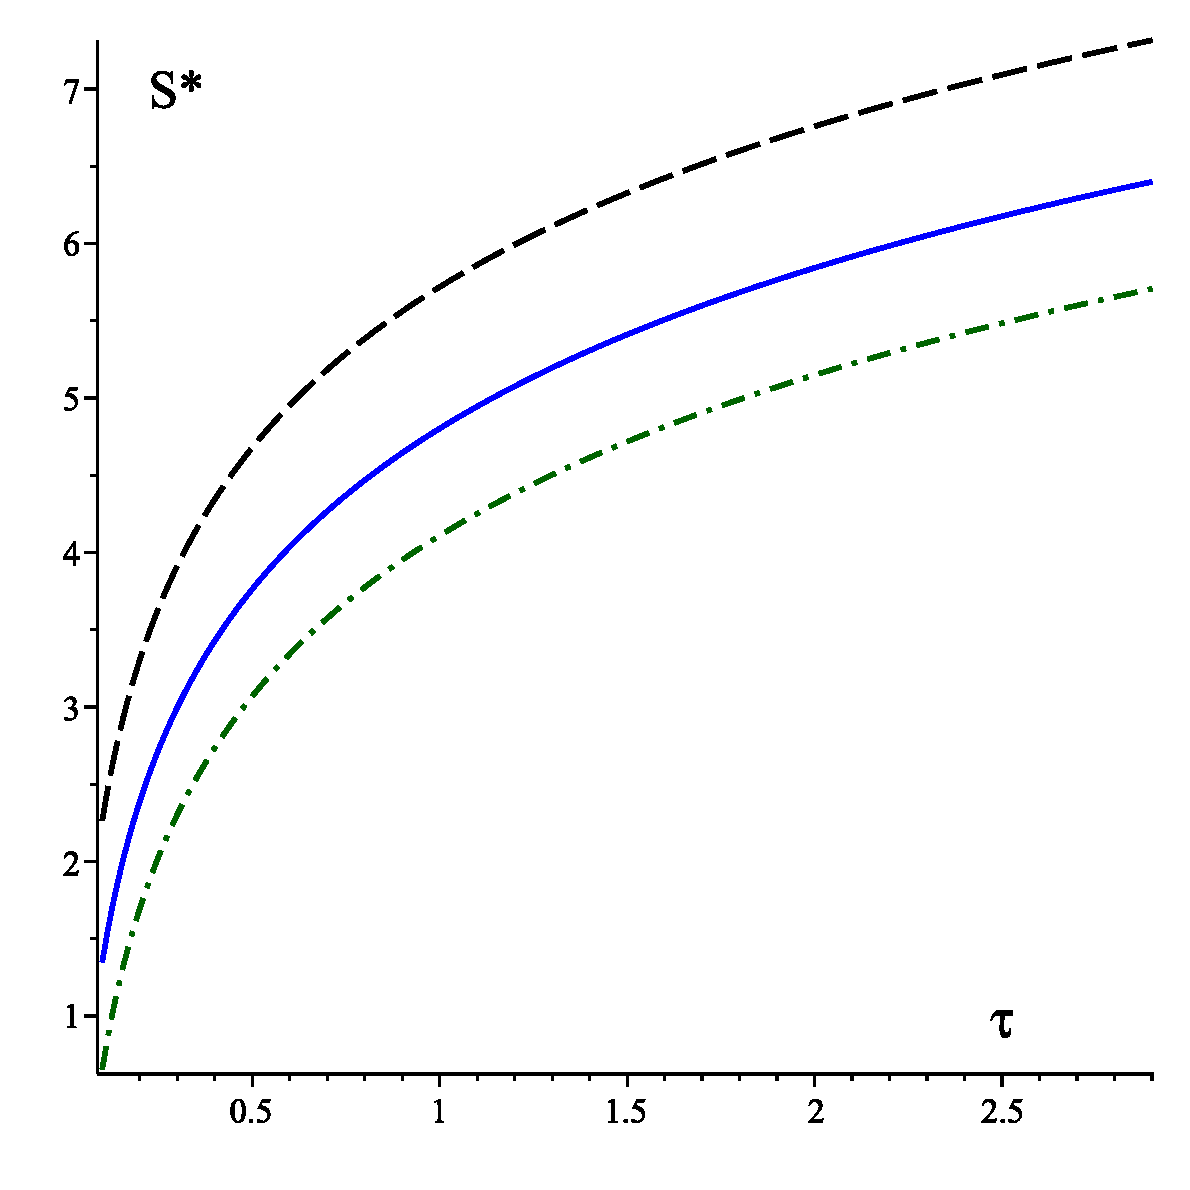
\includegraphics[width=0.4\textwidth,angle=0]{vdw_S_vs_t}
		\hfill
		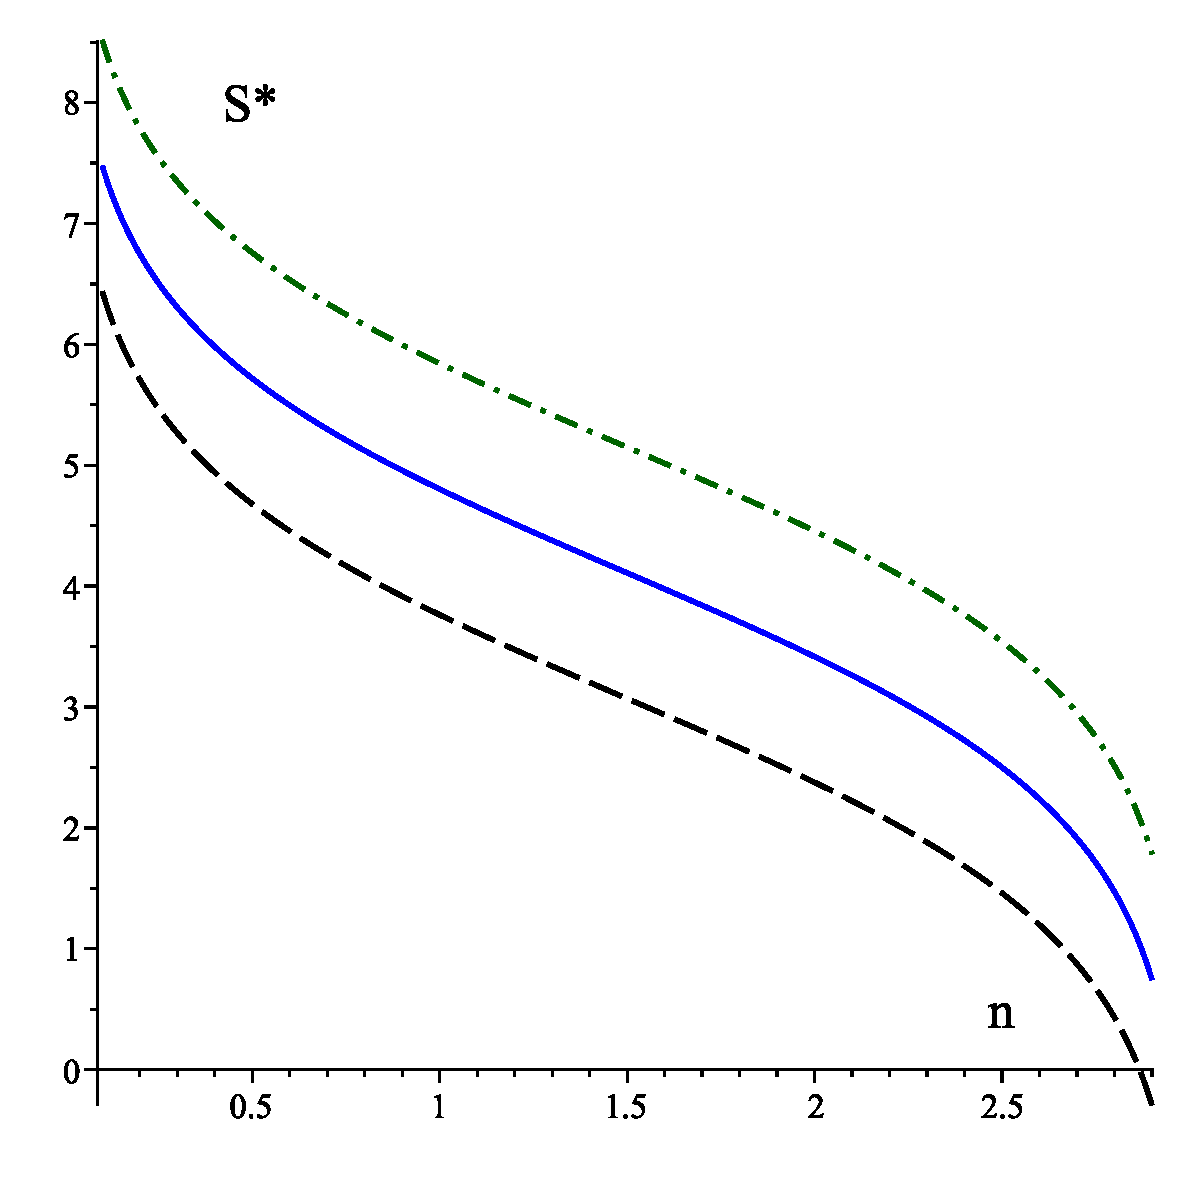
\includegraphics[width=0.4\textwidth,angle=0]{vdw_S_vs_n}
		\\
		%\captionsetup{width=0.5\textwidth}
		\parbox{0.45\textwidth}{\caption{\label{fig:vdw_S_vs_t} Entropy per particle $S^{*}$ of the vdW fluid as a function of temperature $\hat{\tau}$ at a given density. (Dashed black line): $\hat{n}=0.5$, (Solid blue line): $\hat{n}=1.0$, and (Dash-dotted green line): $\hat{n}=1.5$.}}
		\hfill
		%\captionsetup{width=0.5\textwidth}
		\parbox{0.45\textwidth}{\caption{\label{fig:vdw_S_vs_n} Entropy per particle $S^{*}$ of the vdW fluid as a function of density $\hat{n}$ at a given temperature. (Dashed black line): $\hat{\tau}=0.5$, (Solid blue line): $\hat{\tau}=1.0$, and (Dash-dotted green line): $\hat{\tau}=2.0$.}}
	\end{figure}
	
	The chemical potential of the vdW fluid is given by~\cite[(70c)]{Johnston14}
	\begin{equation}
		\label{vdw:mu}
		\frac{\mu}{k_{\rm B}T_c} = -\hat{\tau} \ln \left(\frac{3-\hat{n}}{\hat{n}}\right) + \frac{\hat{\tau}\hat{n}}{3-\hat{n}} - \frac{9\hat{n}}{4} - \hat{\tau}\ln(\hat{\tau}^{3/2}) - \hat{\tau}\ln(x_c).
	\end{equation}
	Considering Eqs.~\eqref{vdw:mu} and~\eqref{vdw:S} together as parametric equation, we can plot dependence of entropy on chemical potential at a given temperature, see Fig.~\ref{fig:vdw_S_vs_mu}.
	
	\begin{figure}[htbp]
		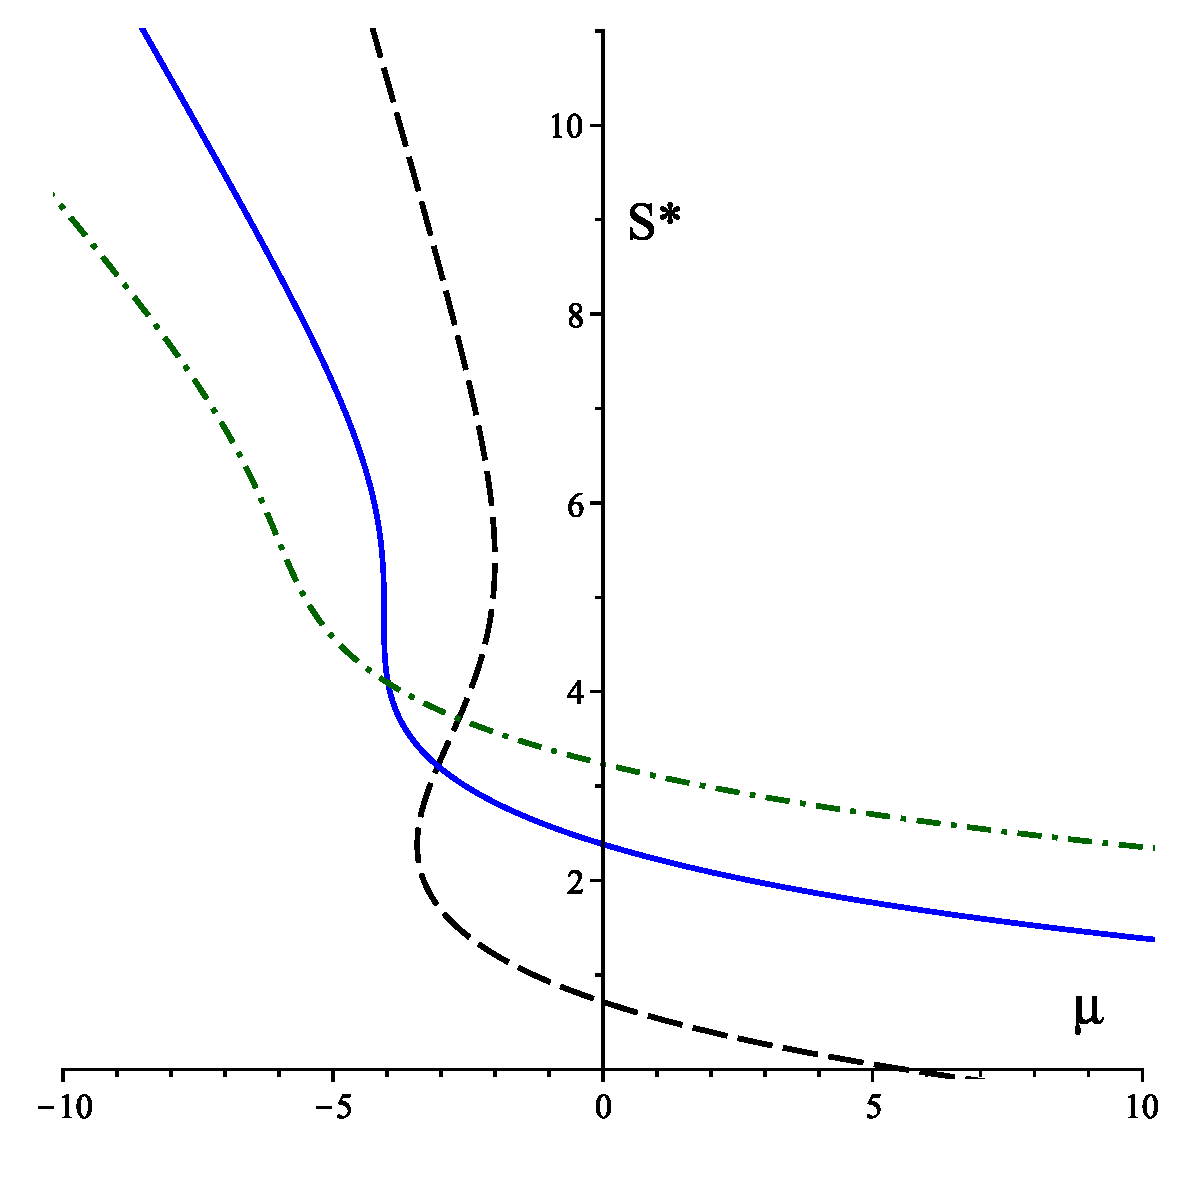
\includegraphics[width=0.45\textwidth,angle=0]{vdw_S_vs_mu}
		\hfill
		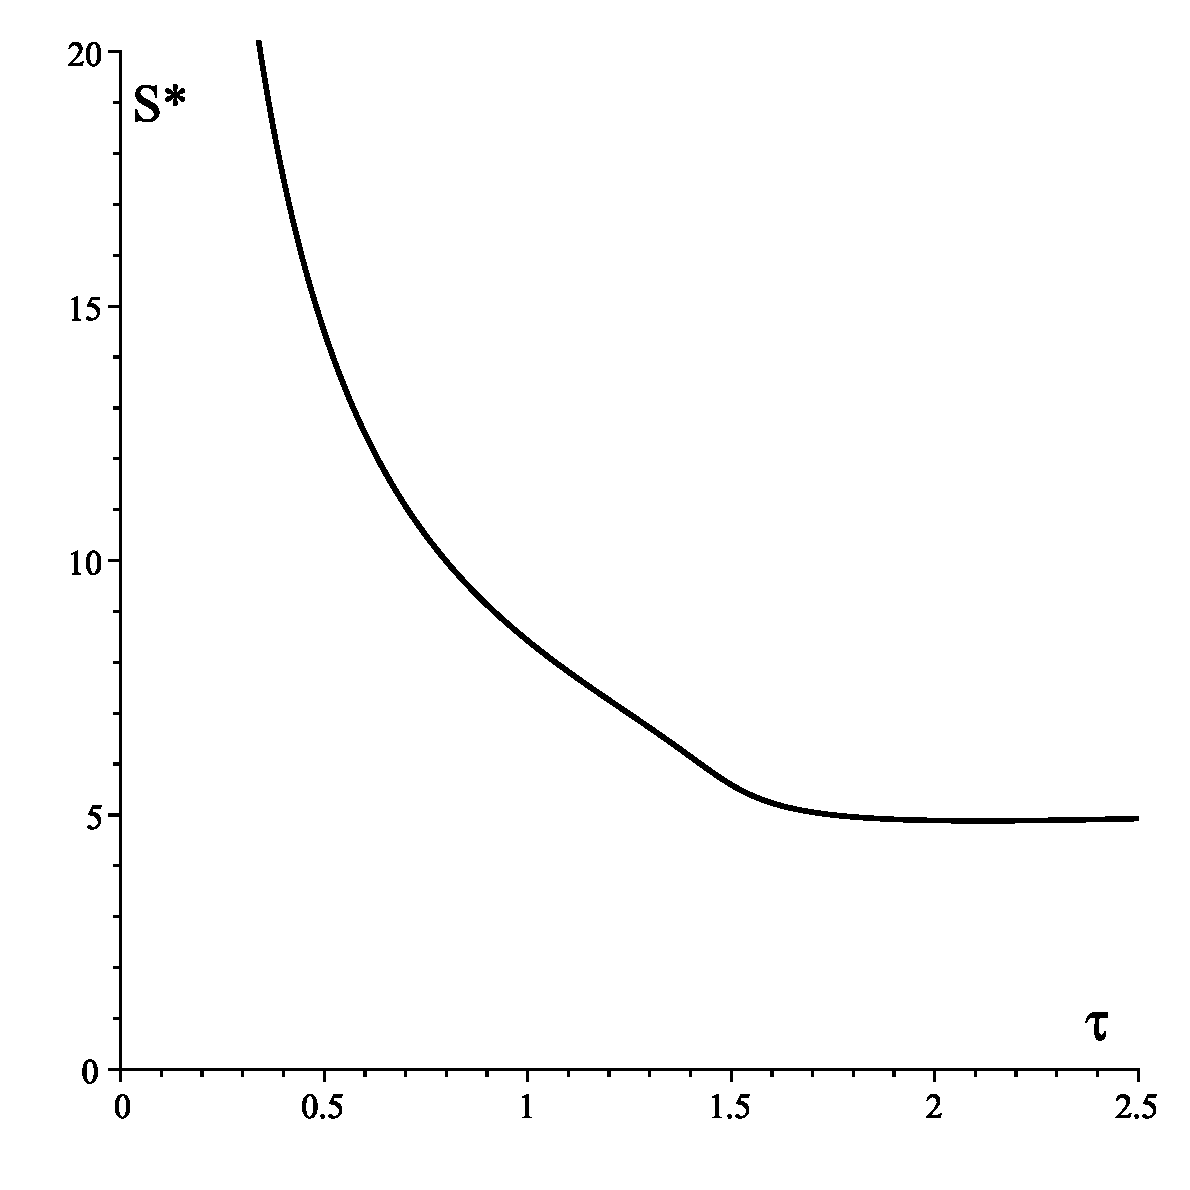
\includegraphics[width=0.45\textwidth,angle=0]{vdw_S_vs_t_at_mu}
		\\
		%\captionsetup{width=0.5\textwidth}
		\parbox{0.45\textwidth}{\caption{\label{fig:vdw_S_vs_mu} Entropy per particle $S^{*}$ of the vdW fluid as a function of chemical potential $\mu/(k_{\rm B}T_c)$ at a given temperature, (Dashed black line): $\hat{\tau}=0.5$, (Solid blue line): $\hat{\tau}=1.0$, (Dash-dotted green line): $\hat{\tau}=1.5$.}}
		\hfill
		%\captionsetup{width=0.5\textwidth}
		\parbox{0.45\textwidth}{\caption{\label{fig:vdw_S_vs_t_at_mu} Entropy per particle $S^{*}$ of the vdW fluid as a function of temperature $\hat{\tau}$ at a given chemical potential $\mu/(k_{\rm B}T_c) = -6.0$.}}
	\end{figure}
	
	\pagebreak
	\section{Notation}

---

$V$ - volume;

$N_v$ - number of cubic cells in the whole volume $V$;

$\Delta_{l}$ - a cubic cell; the $l$-th cubic cell;

$c$ - linear size of a cubic cell.

$v \equiv c^3$ - volume of a cubic cell.

$\gamma$ - configuration of particles;

$\vb r$; $\vb{r}'$ - coordinate in three-dimensional space;

$r \equiv \abs{\vb r}$ - absolute value of $\vb r$;

$\vb{r}_i$ - space coordinate of the $i$-th particle;

$\vb{r}^N \equiv \vb{r}_1, ..., \vb{r}_N$ - space coordinates of particles in a configuration $\gamma$;

$N$; $\abs{\gamma}$ - number of particles in a configuration $\gamma$;

$\Phi_{N_v}(\vb{r}_i, \vb{r}_j)$ - interaction potential between particles (the Curie-Weiss potential);

$J_1$ - characteristic energy for attraction;

$J_2$ - characteristic energy for repulsion;

$a \equiv J_2/J_1$ - ratio between attraction and repulsion characteristic energies;

$W_{N_v}(\gamma)$; $W_{N_v}(\vb{r}^N)$ - potential energy of the interparticle interaction in $\gamma$;

$\mathbb{I}_{\Delta_l} (\vb{r})$ - indicator function for a cell $\Delta_{l}$;

$\gamma_l = \gamma \cap \Delta_l$ - a part of $\gamma$ contained in $\Delta_l$;

$N_l$; $\abs{\gamma_l}$ - number of particles in $\gamma_l$;

---

$\Xi$ - grand partition function;

$\zeta$ - activity;

$\beta$ - inverse temperature;

$k_{\rm B}$ - Boltzmann constant;

$T$ - temperature;

$\mu$ - chemical potential;

$\Lambda$ - de Broglie thermal wavelength;

$\hbar$ - Planck constant;

$m$ - mass of a particle;

$Z_N$ - configuration integral;

${\rm d} \vb{r}^N \equiv {\rm d}{\vb r_1} \dotsc {\rm d}{\vb r_N}$;

$\langle\ldots\rangle$ - average over the grand canonical distribution;

$\Omega = -k_{\rm B}T \ln \Xi$ - grand potential;

---

$T^* \equiv \frac{k_{\rm B}T}{J_1}$ - reduced temperature.

$\beta^* \equiv \beta J_1 = 1/T^*$; $p \equiv \beta J_1 = 1/T^*$ - reduced inverse temperature;

$\mu^* \equiv \frac{\mu}{J_1}$ - reduced chemical potential;

$P$ - pressure;

$P^* \equiv \frac{Pv}{J_1}$ - reduced pressure;

$\rho$ - particle density;

$\rho^* \equiv \frac{\langle N \rangle}{V}v$ - reduced particle density;

$S$ - entropy;

$S^* \equiv \frac{S}{k_{\rm B} \langle N \rangle}$ - reduced entropy;

$Q_c$ - critical value of a quantity $Q$ (may be any of listed above);

$v^* \equiv {v}/{\Lambda_c^3}$ - dimensionless cell volume;

---

$\delta_{nm}$ - Kronecker $\delta$-symbol;

$l$; $l'$ - index for a cubic cell;

$i$; $j$ - index for a particle;

$\mathbb{N}$ - set of natural numbers;

$\mathbb{N}_0$ - set of non-negative integer numbers;

$\mathbb{R}$ - set of real numbers;

$\varrho \in \mathbb{N}_0^{N_v}$; $\varrho = (\varrho_1, \varrho_2, \ldots, \varrho_{N_{v}})$ - vector with non-negative integer components;

$\nu(\gamma)=(N_1, N_2, \ldots, N_{N_v})$; $\nu(\gamma) = (\abs{\gamma_1}, \abs{\gamma_2}, \ldots, \abs{\gamma_{N_v}})$ - vector representing number of particles in each cell;

---

$f(n; \lambda)$ - non-normalized Poisson distribution;

$\lambda$ - parameter of the Poisson distribution;

$K_n(T^*,\mu^*;y)$ - special functions.

$E(T^*,\mu^*;y)$, $E_1(T^*,\mu^*;y)$, $E_2(T^*,\mu^*;y)$ - quantities defined in~\eqref{def:reducedE}, \eqref{def:reducedE1}, \eqref{def:reducedE2}, respectively.

$\bar{y} = \bar{y}(T^*,\mu^*)$ - function that maximizes $E(T^*,\mu^*;y)$.



\section*{Abbreviations}
---

GPF - Grand Partition Function;

CW - Curie-Weiss

	\pagebreak	
	%\bibliographystyle{elsarticle-num}
	%\bibliography{books,articles}
	
	\bibliographystyle{JHEPm}
	\bibliography{Mbank}
		
\end{document} 
